\section{\trInfinityCategories{}}
\label{sec:infinity-categories}

本节我们将朝着\trInfinityCategories{}的定义迈进，并以\cref{thm:spine-horn-nerve}%
为动机。这自然地引出两种（分属先验与后验的）不同的可行定义，其中较为朴素的那个
在本书中称为\emph{\trComposer{}}（composer）。我们将阐明为什么由\trJoyal{}定义的%
\trInfinityCategory{}概念比\trComposer{}的概念表现更好，以及这一点如何使它成为普通%
\trCategory{}的「正确」推广。此外，我们还将讨论\trInfinityCategories{}的若干例子
以及可对其实施的一些基本运算。构造\trInfinityCategories{}的一件「引入%
工具」\footnote{译注：原书此处作「import tool」（引入工具），疑为「important
tool」（重要工具）之误。}是单纯\trEnrichment{}范畴（simplicially enriched category），因此
我们将稍稍绕道，按我们的目的之所需讨论\trEnrichment{}范畴。

\begin{definition}\label{def:composer}
\emph{\trComposer{}}是具有对\trSpine{}包含 $I^n \to \Delta^n$ 的扩张性质的\trSimplicialSet{}。
\end{definition}

\begin{definition}\label{def:composer-objects-morphisms}
在一个\trComposer{}中（事实上，在一般的\trSimplicialSet{}中），我们把 $0$-\trSimplex{}称为%
\emph{\trObject{}}，并把 $1$-\trSimplex{} $f$ 称为从 $d_1(f)$（\trSource{}）到 $d_0(f)$（\trTarget{}）的一个%
\emph{\trMorphism{}}。我们把对象 $x$ 的恒等\trMorphism{}定义为 $s_0(x)$。对\trComposer{}而言，我们把 $n$ 个可
合成\trMorphism{}的一个\emph{合成}定义为到 $\Delta^n$ 的一个扩张的
选取，有时也仅指到边 $\Delta^{\{0,n\}} \subseteq \Delta^n$ 的限制。
\end{definition}

由这个定义显见，「\trComposer{}」这一名称源于人们\emph{能够}合成\trMorphism{}这一事实。
为避免结合性问题，\trComposer{}配备的是一种 $n$ 元合成律。

\begin{example*}
一个\trTopologicalSpace{}的\trSingularSimplicialSet{}是一个\trComposer{}：%
\trObject{}为各个点，从 $x$ 到 $y$ 的\trMorphism{}为道路。\trMorphism{}的一个合成
就是与诸道路的拼接相对端点\trHomotopy{}的任一条道路。
\end{example*}

\begin{definition}\label{def:equivalent-1-simplices}
设 $X$ 是一个\trSimplicialSet{}。若存在 $2$-\trSimplex{} $\sigma\colon \Delta^2 \to X$
满足以下条件，则称从 $x$ 到 $y$ 的两个 $1$-\trSimplex{} $f$ 与 $g$ 为\emph{等价的}：
\begin{enumerate}[label=(\arabic*)]
  \item $\sigma|_{\Delta^{\{0,1\}}} = f$；
  \item $\sigma|_{\Delta^{\{0,2\}}} = g$；
  \item $\sigma|_{\Delta^{\{1,2\}}} = \mathrm{id}_y$。
\end{enumerate}
\end{definition}

\begin{observation}\label{obs:equivalence-relation-reflexive}
这个关系显然是自反的，但同样地，先验地说它既不传递也不对称。你能否为\trComposer{}再找
出一个提升判据，使得这个关系实际上成为一个等价关系？
\end{observation}

\begin{definition}\label{def:homotopy-category}
设 $X$ 是一个\trSimplicialSet{}。我们用生成元与关系来定义一个\trCategory{} $hX$：
\trObject{}由 $X_0$ 给出；\trMorphism{}由 $X_1$ 生成，也就是说，对每个 $1$-\trSimplex{}%
$f\colon \Delta^1 \to X$ 有一个从 $d_1(f)$ 到 $d_0(f)$ 的\trMorphism{}；自由的
合成记作 $f \star g$。现在我们开始强加关系：
\begin{enumerate}[label=(\arabic*)]
  \item $1$-\trSimplex{} $s_0(x)$ 是 $x$ 的恒等元；
  \item 对每个边界由三元组 $(f, g, h)$ 给出的 $2$-\trSimplex{}%
  $\sigma\colon \Delta^2 \to X$，我们强加关系 $h = g \star f$；
  \item 若 $f \sim f'$，则 $f \star g \sim f' \star g$ 且
  $g' \star f \sim g' \star f'$。
\end{enumerate}
范畴 $hX$ 称为 $X$ 的\emph{\trHomotopy{}范畴}。
\end{definition}

\begin{remark}\label{rem:homotopy-category-functorial}
这个构造显然是\trFunctor{}性的，也就是说，我们有一个\trFunctor{}%
$h\colon \mathrm{sSet} \to \mathrm{Cat}$。
\end{remark}

\begin{lemma}\label{lem:homotopy-category-skeleton}
设 $f\colon X \to Y$ 是一个诱导同构 $\mathrm{sk}_2(X) \to \mathrm{sk}_2(Y)$ 的%
\trSimplicialSet{}之间的映射。那么诱导的映射 $hX \to hY$ 是\trCategory{}之间的一个
同构。
\end{lemma}

\begin{proof}
整个构造只涉及 $X$ 的 $2$-\trSkeleton{}。换言之，由 $h$ 的\trFunctor{}性所诱导的显然映射
$h(\mathrm{sk}_2(X)) \to hX$ 是一个同构。除此之外，我们还需用到如下图表交换这一
事实：
\begin{center}
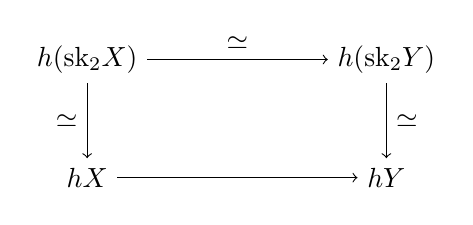
\begin{tikzpicture}
  \node (a) at (0,0) {$h(\mathrm{sk}_2 X)$};
  \node (b) at (3.8,0) {$h(\mathrm{sk}_2 Y)$};
  \node (c) at (0,-1.5) {$hX$};
  \node (d) at (3.8,-1.5) {$hY$};
  \draw[->] (a) -- node[above] {$\simeq$} (b);
  \draw[->] (a) -- node[left] {$\simeq$} (c);
  \draw[->] (b) -- node[right] {$\simeq$} (d);
  \draw[->] (c) -- (d);
\end{tikzpicture}
\end{center}
\end{proof}

\begin{observation}\label{obs:composer-hx-quotient}
一般地，$hX$ 中的\trMorphism{}是 $1$-\trSimplex{}的形式合成（\trSource{}与\trTarget{}正确者）。若 $X$ 是一个%
\trComposer{}，那么我们看到 $hX$ 的\trMorphism{}之集是 $1$-\trSimplex{}之集的一个商，而且同两个%
\trMorphism{}的任何两个合成都会被等同。特别地，等价的\trMorphism{}会被等同：如果我
们有一个 $2$-\trSimplex{}%
\begin{center}
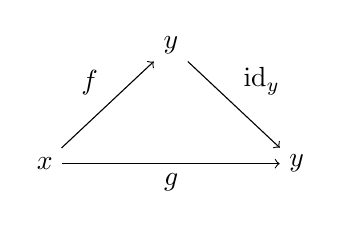
\begin{tikzpicture}
  \node (x) at (0,0) {$x$};
  \node (yt) at (1.6,1.5) {$y$};
  \node (yb) at (3.2,0) {$y$};
  \draw[->] (x) -- node[above left] {$f$} (yt);
  \draw[->] (x) -- node[below] {$g$} (yb);
  \draw[->] (yt) -- node[above right] {$\mathrm{id}_y$} (yb);
\end{tikzpicture}
\end{center}
那么我们发现 $g \sim \mathrm{id}_y \star f \sim f$。
\end{observation}

\begin{lemma}\label{lem:composer-inner-3-horn}
设\trComposer{} $X$ 此外还具有对内 $3$-\trHorn{}包含的提升性质。设 $f$ 与 $g$ 是 $X$ 中可
合成的 $1$-\trSimplex{}。那么：
\begin{enumerate}[label=(\arabic*)]
  \item 存在 $f$ 与 $g$ 的一个合成；
  \item \cref{def:equivalent-1-simplices} 意义下\trMorphism{}的「等价」关系是一个等价
  关系；
  \item $f$ 与 $g$ 的任何两个合成在\cref{def:equivalent-1-simplices} 的意义下等价；并且
  \item 给定 $2$-\trSimplex{} $\sigma$，使得 $\sigma_{\Delta^{\{0,1\}}} = \mathrm{id}_x$、
  $\sigma_{\Delta^{\{1,2\}}} = h$ 且 $\sigma_{\Delta^{\{0,2\}}} = h'$，则
  $h' \sim h$。
\end{enumerate}
\end{lemma}

\begin{proof}
（1）由\trComposer{}的定义得出。对于（2），我们需要证明对称性与传递性。让我们先证对称性。
为此，设 $f, g\colon x \to y$ 是满足 $f \sim g$ 的\trMorphism{}。取 $2$-\trSimplex{}%
$\sigma$，使得 $\sigma_{\Delta^{\{0,1\}}} = f$、$\sigma_{\Delta^{\{0,2\}}} = g$ 且
$\sigma_{\Delta^{\{1,2\}}} = \mathrm{id}_y$。连同 $s_1(f)$ 与 $s_0(\mathrm{id}_y)$
一起，这就确定了一个映射 $\Lambda^3_1 \to X$：
\begin{center}
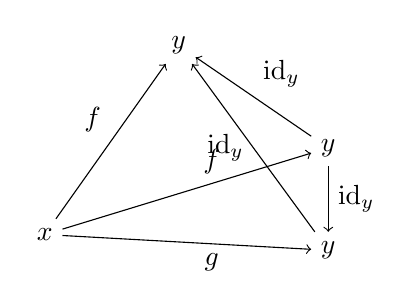
\begin{tikzpicture}
  \node (x) at (0,0) {$x$};
  \node (yt) at (1.7,2.4) {$y$};
  \node (yr) at (3.6,1.1) {$y$};
  \node (yb) at (3.6,-0.2) {$y$};
  \draw[->] (x) -- node[above left] {$f$} (yt);
  \draw[->] (x) -- node[pos=0.6, above] {$f$} (yr);
  \draw[->] (x) -- node[pos=0.6, below] {$g$} (yb);
  \draw[->] (yr) -- node[above right] {$\mathrm{id}_y$} (yt);
  \draw[->] (yb) -- node[left] {$\mathrm{id}_y$} (yt);
  \draw[->] (yr) -- node[right] {$\mathrm{id}_y$} (yb);
\end{tikzpicture}
\end{center}
由于 $X$ 对内 $3$-\trHorn{}具有扩张性质，故存在到 $\Delta^3$ 的一个扩张，它可以限制
到面 $\Delta^{\{0,2,3\}}$ 上。这个 $2$-\trSimplex{}见证了 $g \sim f$。

为了证明传递性，设 $f \sim g \sim h$。取见证这些关系的 $2$-\trSimplex{} $\sigma$ 与
$\sigma'$。连同 $s_0(\mathrm{id}_y)$ 一起，它们定义了一个映射
$\Lambda^3_2 \to X$：
\begin{center}
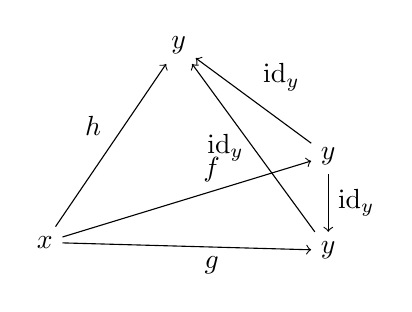
\begin{tikzpicture}
  \node (x) at (0,0) {$x$};
  \node (yt) at (1.7,2.5) {$y$};
  \node (yr) at (3.6,1.1) {$y$};
  \node (yb) at (3.6,-0.1) {$y$};
  \draw[->] (x) -- node[above left] {$h$} (yt);
  \draw[->] (x) -- node[pos=0.6, above] {$f$} (yr);
  \draw[->] (x) -- node[pos=0.6, below] {$g$} (yb);
  \draw[->] (yr) -- node[above right] {$\mathrm{id}_y$} (yt);
  \draw[->] (yb) -- node[left] {$\mathrm{id}_y$} (yt);
  \draw[->] (yr) -- node[right] {$\mathrm{id}_y$} (yb);
\end{tikzpicture}
\end{center}
扩张到 $\Delta^3$ 再限制到 $\Delta^{\{0,1,3\}}$，便表明 $f \sim h$。为了证明（3），
设 $f\colon x \to y$ 与 $g\colon y \to z$ 是可合成的\trMorphism{}。选取合成 $h$ 与
$h'$，连同 $s_1(g)$ 一起，便确定了一个映射 $\Lambda^3_1 \to X$：%
\footnote{译注：下图中间那条边在原书中标作 $\mathrm{id}_y$，但其两端均为 $z$，疑为
$\mathrm{id}_z$ 之误。}
\begin{center}
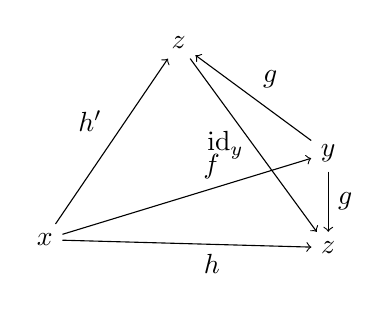
\begin{tikzpicture}
  \node (x) at (0,0) {$x$};
  \node (zt) at (1.7,2.5) {$z$};
  \node (y) at (3.6,1.1) {$y$};
  \node (zb) at (3.6,-0.1) {$z$};
  \draw[->] (x) -- node[above left] {$h'$} (zt);
  \draw[->] (x) -- node[pos=0.6, above] {$f$} (y);
  \draw[->] (x) -- node[pos=0.6, below] {$h$} (zb);
  \draw[->] (y) -- node[above right] {$g$} (zt);
  \draw[->] (zt) -- node[left] {$\mathrm{id}_y$} (zb);
  \draw[->] (y) -- node[right] {$g$} (zb);
\end{tikzpicture}
\end{center}
扩张到 $\Delta^3$ 再限制到 $\Delta^{\{0,1,3\}}$，便表明 $h \sim h'$。为了证明（4），
我们考虑由如下图表给出的映射 $\Lambda^3_2 \to X$
\begin{center}
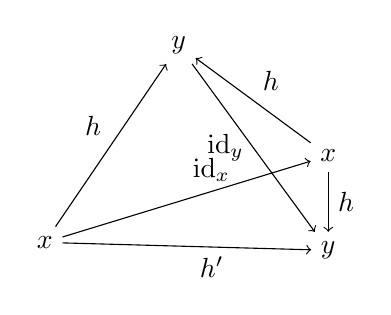
\begin{tikzpicture}
  \node (x) at (0,0) {$x$};
  \node (yt) at (1.7,2.5) {$y$};
  \node (xr) at (3.6,1.1) {$x$};
  \node (yb) at (3.6,-0.1) {$y$};
  \draw[->] (x) -- node[above left] {$h$} (yt);
  \draw[->] (x) -- node[pos=0.6, above] {$\mathrm{id}_x$} (xr);
  \draw[->] (x) -- node[pos=0.6, below] {$h'$} (yb);
  \draw[->] (xr) -- node[above right] {$h$} (yt);
  \draw[->] (yt) -- node[left] {$\mathrm{id}_y$} (yb);
  \draw[->] (xr) -- node[right] {$h$} (yb);
\end{tikzpicture}
\end{center}
并把它扩张到 $\Delta^3$。把结果限制到 $\Delta^{\{0,2,3\}}$ 便表明 $h' \sim h$。
\end{proof}

\begin{lemma}\label{lem:pi-x-category}
设 $X$ 是具有内 $3$-\trHorn{}扩张性质的\trComposer{}。那么存在一个\trCategory{} $\pi(X)$，
其\trObject{}由 $X$ 的 $0$-\trSimplex{}给出，而其\trMorphism{}由 $X$ 中 $1$-\trSimplex{}的等价类
（在\cref{def:equivalent-1-simplices} 的意义下）给出。合成经由沿 $I^2 \to \Delta^2$
的提升来定义。合成的唯一性（在等价的意义下）表明 $\pi(X)$ 中的合成是结合的。
\end{lemma}

\begin{proof}
只剩下证明合成是结合的了。为此，只需证明：若 $f$、$g$、$h$ 是可合成的\trMorphism{}，
则 $h \circ (gf)$ 是 $hg$ 与 $f$ 的一个合成。考虑由如下图表给出的映射
$\Lambda^3_1 \to X$：%
\footnote{译注：按正文「可合成的\trMorphism{} $f$、$g$、$h$」，一般应有
$h\colon z \to w$（$w$ 可异于 $z$）；原书图中 $h$ 的两端均标作 $z$，此处照实复刻。}
\begin{center}
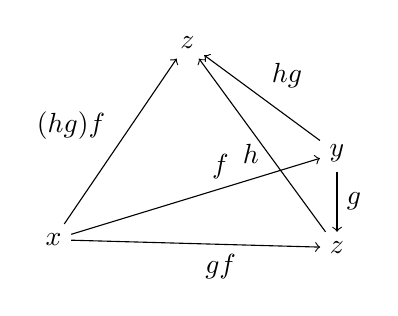
\begin{tikzpicture}
  \node (x) at (0,0) {$x$};
  \node (zt) at (1.7,2.5) {$z$};
  \node (y) at (3.6,1.1) {$y$};
  \node (zb) at (3.6,-0.1) {$z$};
  \draw[->] (x) -- node[pos=0.45, above left] {$(hg)f$} (zt);
  \draw[->] (x) -- node[pos=0.6, above] {$f$} (y);
  \draw[->] (x) -- node[pos=0.6, below] {$gf$} (zb);
  \draw[->] (y) -- node[above right] {$hg$} (zt);
  \draw[->] (zb) -- node[pos=0.45, left] {$h$} (zt);
  \draw[->] (y) -- node[right] {$g$} (zb);
\end{tikzpicture}
\end{center}
扩张到 $\Delta^3$ 再限制到 $\Delta^{\{0,2,3\}}$，便表明 $(hg)f$ 是 $gf$ 与 $h$ 的一个
合成。由于 $X$ 中的合成在等价的意义下唯一，$\pi(X)$ 中合成的结合性随之得证。
\end{proof}

\begin{corollary}\label{cor:hx-pi-x}
设 $X$ 是具有内 $3$-\trHorn{}提升性质的\trComposer{}。那么 $hX$ 同构于 $\pi(X)$。特别地，
对带有附加内 $3$-\trHorn{}提升条件的\trComposer{}而言，$X$ 的\trHomotopy{}范畴有一个非常
显式的描述。
\end{corollary}

\begin{proof}
存在一个典范\trFunctor{} $hX \to \pi(X)$，其构造如下：它在\trObject{}上是恒等的，并
由 $1$-\trSimplex{}上的恒等所诱导。由于在 $hX$ 中强加的所有关系在 $\pi(X)$ 中都成立，这事实
上便给出所需的\trFunctor{}。只需证明：对任意两个\trObject{} $x, y \in X$，典范映射
\[
\mathrm{Hom}_{hX}(x, y) \to \mathrm{Hom}_{\pi(X)}(x, y)
\]
是双射。为了说明这一点，我们观察到存在交换图表
\begin{center}
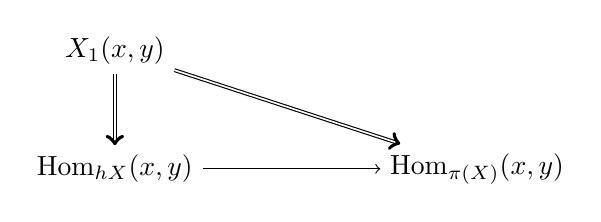
\begin{tikzpicture}
  \node (x1) at (0,0) {$X_1(x, y)$};
  \node (h) at (0,-1.5) {$\mathrm{Hom}_{hX}(x, y)$};
  \node (p) at (4.6,-1.5) {$\mathrm{Hom}_{\pi(X)}(x, y)$};
  \draw[double, ->] (x1) -- (h);
  \draw[double, ->] (x1) -- (p);
  \draw[->] (h) -- (p);
\end{tikzpicture}
\end{center}
其中 $X_1(x, y)$ 表示满足 $d_1(f) = x$ 且 $d_0(f) = y$ 的 $1$-\trSimplex{} $f$ 之集。多亏
$\pi$ 的定义与\cref{obs:composer-hx-quotient}，从 $X_1(x, y)$ 出发的两个映射都是满
射，因此水平映射是满射。剩下要证这个映射也是单射。为此，假设给定了两个在 $\pi(X)$
中像相同的\trMorphism{} $f, g \in X_1(x, y)$。这意味着它们在%
\cref{def:equivalent-1-simplices} 的意义下等价。但再次由%
\cref{obs:composer-hx-quotient}，这意味着 $f \sim g$。
\end{proof}

\begin{remark}\label{rem:weak-composer}
在上面的推论中，$X$ 其实不必是\trComposer{}，而只需能对 $2$ 个可合成的\trMorphism{}作出
合成。在后文中，我们把具有对 $2$-脊（即内 $2$-\trHorn{}）的扩张性质的%
\trSimplicialSet{}称为\emph{\trWeakComposer{}}（weak composer）。为了同时合成许多%
\trMorphism{}，我们归纳地进行合成，并在等价的意义下得到一个良定义的「$n$ 重合成」
（只要该\trWeakComposer{}也满足对内 $3$-\trHorn{}的扩张性质）。
\end{remark}

现在注意 $I^2 = \Lambda^2_1$。因此，我们可以把上述陈述重述如下：

\begin{corollary}\label{cor:hx-iso-pi-x}
设 $X$ 是一个对内 $2$-与 $3$-\trHorn{}均容许提升的\trSimplicialSet{}。那么 $hX$ 同构
于 $\pi(X)$。
\end{corollary}

\begin{corollary}\label{cor:h-nerve-iso}
设 $\C$ 是一个\trCategory{}。那么 $h(\mathrm{N}(\C))$ 典范地同构于 $\C$。
\end{corollary}

\begin{proof}
我们已经看到 $\mathrm{N}(\C)$ 对许多\trHorn{}容许（唯一的）提升，其中包括上一个推论
中所描述的那些。因此，只需证明 $\pi(\mathrm{N}(\C)) \cong \C$。但我们回顾一下，
$\mathrm{N}(\C)$ 中\trMorphism{}的「等价」关系就是「相等」关系。
\end{proof}

\begin{definition}\label{def:infinity-category}
一个\trSimplicialSet{}称为\emph{\trInfinityCategory{}}，若它对所有内\trHorn{}包含
$\Lambda^n_j \to \Delta^n$（$n \ge 2$，$0 < j < n$）具有扩张性质。
\end{definition}

\begin{definition}\label{def:functor-infinity-categories}
两个\trInfinityCategories{}之间的一个\trFunctor{}恰好就是\trSimplicialSet{}之间的一个
映射。换言之，\trInfinityCategories{}的\trCategory{}是 $\mathrm{sSet}$ 中由那些为%
\trInfinityCategories{}的对象组成的满子范畴。
\end{definition}

在本书的后续阶段，我们会看到，非正式地说，一个\trInfinityCategory{}是一个\trComposer{}，
其中合成的选取在相差一个可缩选取空间的意义下唯一：对\trComposer{} $X$ 中每一对可合成的%
\trMorphism{} $f$ 与 $g$，都有一个由 $f$ 与 $g$ 的合成构成的\trSimplicialSet{}%
$\mathrm{Comp}_X(f, g)$，它由如下\trPullback{}给出
\begin{center}
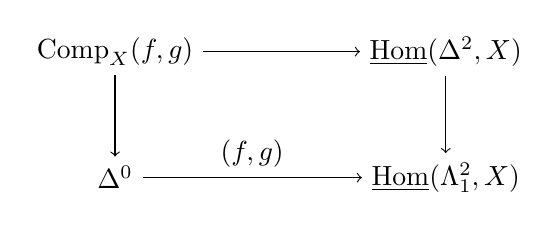
\begin{tikzpicture}
  \node (c) at (0,0) {$\mathrm{Comp}_X(f, g)$};
  \node (h2) at (4.2,0) {$\underline{\mathrm{Hom}}(\Delta^2, X)$};
  \node (d0) at (0,-1.6) {$\Delta^0$};
  \node (h1) at (4.2,-1.6) {$\underline{\mathrm{Hom}}(\Lambda^2_1, X)$};
  \draw[->] (c) -- (h2);
  \draw[->] (c) -- (d0);
  \draw[->] (h2) -- (h1);
  \draw[->] (d0) -- node[above] {$(f, g)$} (h1);
\end{tikzpicture}
\end{center}
根据\cref{ex:composition-space-connected}，内 $3$-\trHorn{}提升条件告诉我们 $\mathrm{Comp}_X(f, g)$ 是连通的，也就
是说，它的 $\pi^{\Delta}_0(-)$ 为零。如果我们现在进而要求 $X$ 确实对所有
$\Lambda^n_j \to \Delta^n$ 的内\trHorn{}包含具有扩张性质，那么我们就得到下面两个
事实（我们将在后文证明）：
\begin{enumerate}[label=(\arabic*)]
  \item \trSimplicialSet{} $\mathrm{Comp}_X(f, g)$ 是一个\trKanComplex{}；
  \item \emph{所有}单纯\trHomotopy{}群 $\pi^{\Delta}_n(\mathrm{Comp}_X(f, g))$ 都
  为零。
\end{enumerate}
因此，一个\trInfinityCategory{}是一个\trComposer{}，其中合成在相差一个可缩选取空间的意义
下是良定义的。

\begin{example*}
一个\trKanComplex{}——从而空间 $X$ 的\trSingularSimplicialSet{} $\mathcal{S}(X)$——
是一个\trInfinityCategory{}。此外，任何\trCategory{}的\trNerve{}也是一个%
\trInfinityCategory{}。
\end{example*}

为了比较\trInfinityCategories{}与\trComposer{}，我们陈述下面的命题。其证明将在后文给出，
见命题 1.3.22 与命题 1.3.12。

\begin{proposition}\label{prop:infinity-category-composer}
每个\trInfinityCategory{}都是\trComposer{}。然而，也存在不是\trInfinityCategories{}的\trComposer{}。
\end{proposition}

\begin{proposition}\label{prop:h-n-adjoint}
\trFunctor{}对
\[
h\colon \mathrm{sSet} \rightleftarrows \mathrm{Cat} : \mathrm{N}
\]
是\trAdjunction{}的，其中 $\mathrm{N}$ 是 $h$ 的\trRightAdjoint{}。
\end{proposition}

\begin{proof}
我们需要明确单位与余单位\trNaturalTransformation{}。余单位是同构
\[
h(\mathrm{N}(\C)) \cong \C
\]
即\cref{cor:h-nerve-iso} 中的同构。为了构造一个自然映射 $X \to \mathrm{N}(hX)$，即
该\trAdjunction{}的单位，我们发现它在 $0$-\trSimplex{}与 $1$-\trSimplex{}上有典范的映射：回忆 $hX$ 的%
\trObject{}就是 $X$ 的 $0$-\trSimplex{}，而且有一个从 $X_1$ 到 $hX$ 的\trMorphism{}的典范
映射（当 $X$ 是\trComposer{}时，这个映射是满射）。为了构造一般 $n$-\trSimplex{}上的映射，我们观察
到 $n$-\trSimplex{} $\Delta^n \to \mathrm{N}(hX)$ 由其到\trSpine{}上的限制唯一确定，也就是
说，考虑图表
\begin{center}
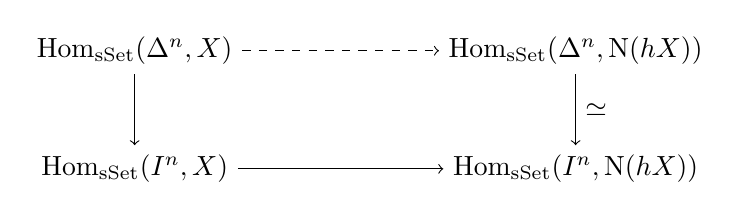
\begin{tikzpicture}
  \node (a) at (0,0) {$\mathrm{Hom}_{\mathrm{sSet}}(\Delta^n, X)$};
  \node (b) at (5.6,0) {$\mathrm{Hom}_{\mathrm{sSet}}(\Delta^n, \mathrm{N}(hX))$};
  \node (c) at (0,-1.5) {$\mathrm{Hom}_{\mathrm{sSet}}(I^n, X)$};
  \node (d) at (5.6,-1.5) {$\mathrm{Hom}_{\mathrm{sSet}}(I^n, \mathrm{N}(hX))$};
  \draw[->, dashed] (a) -- (b);
  \draw[->] (a) -- (c);
  \draw[->] (b) -- node[right] {$\simeq$} (d);
  \draw[->] (c) -- (d);
\end{tikzpicture}
\end{center}
然后，只需使用双射
\[
\mathrm{Hom}_{\mathrm{sSet}}(I^n, X) \cong X_1 \times_{X_0} \dotsb \times_{X_0} X_1
\]
以及 $\mathrm{N}(hX)$ 相应的双射和之前的观察，便可得到一般 $n$-\trSimplex{}上的映射。容易
验证，这些映射事实上是一个\trAdjunction{}的单位与余单位。

或者，你也可以证明由 $h$ 与上述余单位所诱导的映射
\[
\mathrm{Hom}_{\mathrm{sSet}}(X, \mathrm{N}(\C)) \to \mathrm{Fun}(hX, \C)
\]
是双射。这可以由定义立即得出。
\end{proof}

\begin{lemma}\label{lem:adjoint-fully-faithful}
设 $(F, G, \varepsilon, \eta)$ 是一个\trAdjunction{}，其中 $F\colon \C \to \D$
是\trLeftAdjoint{}，$G$ 是\trRightAdjoint{}，$\varepsilon\colon FG \to \mathrm{id}$
是余单位，而 $\eta\colon \mathrm{id} \to GF$ 是单位。那么：
\begin{enumerate}[label=(\arabic*)]
  \item $G$ 是\trFullyFaithful{}当且仅当 $\varepsilon$ 是同构；并且
  \item $F$ 是\trFullyFaithful{}当且仅当 $\eta$ 是同构。
\end{enumerate}
\end{lemma}

\begin{proof}
考虑图表
\begin{center}
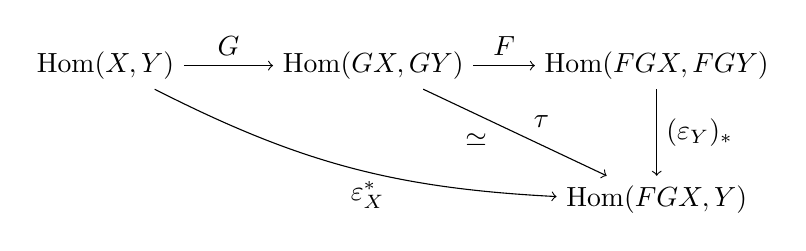
\begin{tikzpicture}
  \node (a) at (0,0) {$\mathrm{Hom}(X, Y)$};
  \node (b) at (3.4,0) {$\mathrm{Hom}(GX, GY)$};
  \node (c) at (7.0,0) {$\mathrm{Hom}(FGX, FGY)$};
  \node (d) at (7.0,-1.7) {$\mathrm{Hom}(FGX, Y)$};
  \draw[->] (a) -- node[above] {$G$} (b);
  \draw[->] (b) -- node[above] {$F$} (c);
  \draw[->] (c) -- node[right] {$(\varepsilon_Y)_*$} (d);
  \draw[->] (b) -- node[pos=0.55, above right] {$\tau$}
    node[pos=0.4, below left] {$\simeq$} (d);
  \draw[->] (a) to[bend right=12] node[pos=0.55, below] {$\varepsilon_X^*$} (d);
\end{tikzpicture}
\end{center}
右边那个三角形交换的事实是\cref{ex:adjunction-unit-counit} 解答的一部分。（事实上，带有双自然同构 $\tau$ 的\trAdjunction{}正是按这种方式翻译成用单位与余单位表述的\trAdjunction{}的。）现在我们断言这个大图表也
交换。具体展开来说，我们需要验证：对每个\trMorphism{} $f\colon X \to Y$，图表
\begin{center}
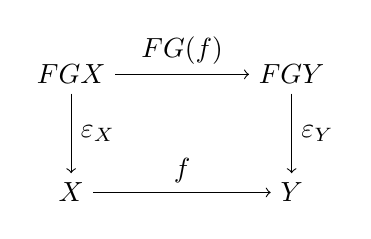
\begin{tikzpicture}
  \node (a) at (0,0) {$FGX$};
  \node (b) at (2.8,0) {$FGY$};
  \node (c) at (0,-1.5) {$X$};
  \node (d) at (2.8,-1.5) {$Y$};
  \draw[->] (a) -- node[above] {$FG(f)$} (b);
  \draw[->] (a) -- node[right] {$\varepsilon_X$} (c);
  \draw[->] (b) -- node[right] {$\varepsilon_Y$} (d);
  \draw[->] (c) -- node[above] {$f$} (d);
\end{tikzpicture}
\end{center}
交换。这是对的，因为 $\varepsilon\colon FG \to \mathrm{id}$ 是\trFunctor{}之间的一个%
\trNaturalTransformation{}。于是我们看到，$G$ 是\trFullyFaithful{}当且仅当对所有
$X, Y \in \D$，映射 $\varepsilon_X^*$ 都是同构。由\trYoneda{}引理，这当且仅当
$\varepsilon_X$ 自身对所有 $X$ 都是同构时成立，这就证明了断言（1）。（2）的论证是
类似的。
\end{proof}

\begin{corollary}\label{cor:nerve-fully-faithful}
\trNerve{}\trFunctor{}是\trFullyFaithful{}。其本质像由\cref{thm:spine-horn-nerve}
描述。\footnote{译注：原书此处称「Proposition 1.1.52」，而第 24 页处作「Theorem
1.1.52」；本书统一按定理 1.1.52 引用。}
\end{corollary}

\begin{proof}
我们在\cref{prop:h-n-adjoint} 中通过构造明确的单位与余单位映射证明了 $\mathrm{N}$
是 $h$ 的\trRightAdjoint{}。于是，由\cref{lem:adjoint-fully-faithful}，只需验证这个\trAdjunction{}的余单位是同构。而由构造，余单位由典范同构 $h(\mathrm{N}(\C)) \to \C$ 给出。
\end{proof}

让我们也记录下下面这个推论，\cref{ex:nerve-2-coskeletal} 要求从定义出发证明它。

\begin{corollary}\label{cor:nerve-2-coskeletal}
\trCategory{}的\trNerve{}是 $2$-\trCoskeleton{}的。
\end{corollary}

\begin{proof}
存在交换图表
\begin{center}
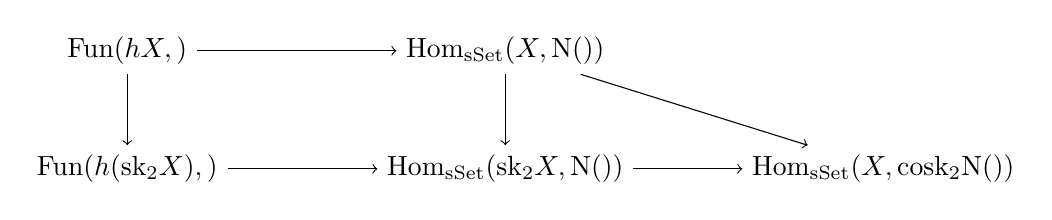
\begin{tikzpicture}
  \node (a) at (0,0) {$\mathrm{Fun}(hX, \C)$};
  \node (b) at (4.8,0) {$\mathrm{Hom}_{\mathrm{sSet}}(X, \mathrm{N}(\C))$};
  \node (c) at (0,-1.5) {$\mathrm{Fun}(h(\mathrm{sk}_2 X), \C)$};
  \node (d) at (4.8,-1.5) {$\mathrm{Hom}_{\mathrm{sSet}}(\mathrm{sk}_2 X, \mathrm{N}(\C))$};
  \node (e) at (9.6,-1.5) {$\mathrm{Hom}_{\mathrm{sSet}}(X, \mathrm{cosk}_2 \mathrm{N}(\C))$};
  \draw[->] (a) -- (b);
  \draw[->] (a) -- (c);
  \draw[->] (b) -- (d);
  \draw[->] (b) -- (e);
  \draw[->] (c) -- (d);
  \draw[->] (d) -- (e);
\end{tikzpicture}
\end{center}
其中斜向箭头由典范映射 $\mathrm{N}(\C) \to \mathrm{cosk}_2 \mathrm{N}(\C)$ 诱导。由
\cref{prop:h-n-adjoint}，左边两个水平映射都是双射，而由%
\cref{lem:homotopy-category-skeleton}，剩下的那个水平箭头也是双射。于是，竖直映射
是双射当且仅当斜向映射是双射。由于 $X$ 是任意的，断言由\trYoneda{}引理得出。
\end{proof}

\begin{definition}\label{def:equivalence-infinity-category}
\trInfinityCategory{}中的一个\trMorphism{}称为一个\emph{\trEquivalence{}}
（equivalence），若它在\trHomotopy{}范畴中的像是同构。
\end{definition}

\begin{lemma}\label{lem:equivalence-2-simplices}
\trInfinityCategory{} $\C$ 中的一个\trMorphism{} $f\colon x \to y$ 是一个%
\trEquivalence{}，当且仅当存在 $2$-\trSimplex{} $\sigma^l\colon \Delta^2 \to \C$ 与
$\sigma^r\colon \Delta^2 \to \C$，使得
\[
\sigma^l|_{\Lambda^2_0} = (f, \mathrm{id})
\quad\text{及}\quad
\sigma^r|_{\Lambda^2_2} = (f, \mathrm{id}).
\]
\end{lemma}

这里，记号 $(g, h)$ 意指第二个\trMorphism{} $h$ 是 $\Delta^2$ 中那个从 $0$ 到 $2$
的\trMorphism{}，而第一个\trMorphism{}在第一种情形是那个从 $0$ 到 $1$ 的，在第二种
情形是那个从 $1$ 到 $2$ 的。

\begin{proof}
若 $2$-\trSimplex{} $\sigma^l$ 存在，则 $\sigma^l|_{\Delta^{\{1,2\}}}$ 是 $f$ 在 $h\C$ 中之像
的一个左逆。类似地，$\sigma^r|_{\Delta^{\{0,1\}}}$ 是 $f$ 在 $h\C$ 中之像的一个右逆。
反之，设 $f$ 的像是 $h\C$ 中的一个\trEquivalence{}。这意味着存在 $1$-\trSimplex{}%
$g\colon y \to x$，使得 $[fg]$ 与 $[gf]$ 是 $h\C$ 中的恒等；也就是说，存在一个
$2$-\trSimplex{} $\eta$ 见证 $h$ 是 $f$ 与 $g$ 的一个合成，并且存在另一个 $2$-\trSimplex{} $\eta'$
见证 $h$ 等价于恒等。我们可以用这两个 $2$-\trSimplex{}（再加上 $g$ 上的一个退化 $2$-\trSimplex{}）
来得到一个映射 $\Lambda^3_2 \to \C$，由于 $\C$ 是\trInfinityCategory{}，它可以被
扩张：
\begin{center}
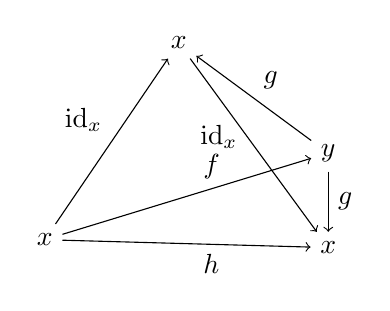
\begin{tikzpicture}
  \node (xbl) at (0,0) {$x$};
  \node (xt) at (1.7,2.5) {$x$};
  \node (y) at (3.6,1.1) {$y$};
  \node (xbr) at (3.6,-0.1) {$x$};
  \draw[->] (xbl) -- node[above left] {$\mathrm{id}_x$} (xt);
  \draw[->] (xbl) -- node[pos=0.6, above] {$f$} (y);
  \draw[->] (xbl) -- node[pos=0.6, below] {$h$} (xbr);
  \draw[->] (y) -- node[above right] {$g$} (xt);
  \draw[->] (xt) -- node[pos=0.45, left] {$\mathrm{id}_x$} (xbr);
  \draw[->] (y) -- node[right] {$g$} (xbr);
\end{tikzpicture}
\end{center}
把所得的 $3$-\trSimplex{}限制到 $2$-\trSimplex{} $\Delta^{\{0,1,3\}}$ 上，便给出一个 $2$-\trSimplex{}%
$\sigma^l$。对 $\sigma^r$ 的论证是类似的。
\end{proof}

\begin{definition}\label{def:infinity-groupoid}
一个\trInfinityCategory{}称为\emph{∞-\trGroupoid{}}（∞-groupoid），若每个%
\trMorphism{}都是一个\trEquivalence{}。
\end{definition}

\begin{definition}\label{def:maximal-sub-infinity-groupoid}
普通\trCategory{}的极大子\trGroupoid{}是由所有同构组成的子范畴，记作
$\C^{\simeq} \subseteq \C$。对一个\trInfinityCategory{} $\C$，我们把极大子∞-\trGroupoid{}%
定义为\trSimplicialSet{}的如下\trPullback{}%
\begin{center}
\begin{tikzpicture}
  \node (a) at (0,0) {$\C^{\simeq}$};
  \node (b) at (3,0) {$\C$};
  \node (c) at (0,-1.5) {$\mathrm{N}(h\C^{\simeq})$};
  \node (d) at (3,-1.5) {$\mathrm{N}(h\C)$};
  \draw[->] (a) -- (b);
  \draw[->] (a) -- (c);
  \draw[->] (b) -- (d);
  \draw[->] (c) -- (d);
\end{tikzpicture}
\end{center}
\end{definition}

\begin{remark}\label{rem:nerve-maximal-groupoid}
对普通\trCategory{} $\C$，我们有 $\mathrm{N}(\C^{\simeq}) = \mathrm{N}(\C)^{\simeq}$，
因为根据定义存在一个\trPullback{}%
\begin{center}
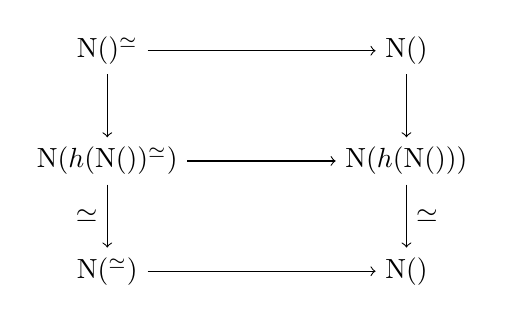
\begin{tikzpicture}
  \node (a) at (0,0) {$\mathrm{N}(\C)^{\simeq}$};
  \node (b) at (3.8,0) {$\mathrm{N}(\C)$};
  \node (c) at (0,-1.4) {$\mathrm{N}(h(\mathrm{N}(\C))^{\simeq})$};
  \node (d) at (3.8,-1.4) {$\mathrm{N}(h(\mathrm{N}(\C)))$};
  \node (e) at (0,-2.8) {$\mathrm{N}(\C^{\simeq})$};
  \node (f) at (3.8,-2.8) {$\mathrm{N}(\C)$};
  \draw[->] (a) -- (b);
  \draw[->] (a) -- (c);
  \draw[->] (b) -- (d);
  \draw[->] (c) -- (d);
  \draw[->] (c) -- node[left] {$\simeq$} (e);
  \draw[->] (d) -- node[right] {$\simeq$} (f);
  \draw[->] (e) -- (f);
\end{tikzpicture}
\end{center}
其中右边竖直映射的复合是恒等，而下面的竖直映射由典范同构
$h(\mathrm{N}(\C)) \cong \C$ 诱导。
\end{remark}

\begin{lemma}\label{lem:maximal-groupoid-edges}
\trInfinityCategory{} $\C$ 的一个 $n$-\trSimplex{} $x$ 属于极大子∞-\trGroupoid{}，当且仅当所有边都是\trEquivalence{}。
\end{lemma}

\begin{proof}
只需观察到 $\mathrm{N}(h\C)$ 中的 $n$-\trSimplex{}由它到所有边上的限制所确定，而且这个
$n$-\trSimplex{}属于 $\mathrm{N}(h\C^{\simeq})$ 当且仅当所有边都是 $h\C$ 中的同构。
\end{proof}

\begin{corollary}\label{cor:maximal-groupoid-infinity-groupoid}
一个\trInfinityCategory{}的极大子∞-\trGroupoid{}事实上是一个∞-\trGroupoid{}，而且它是位于
所给\trInfinityCategory{}之内的最大的这样一个∞-\trGroupoid{}。
\end{corollary}

\begin{proof}
让我们首先证明 $\C^{\simeq}$ 是一个\trInfinityCategory{}。为此，考虑\trLiftingProblem{}%
\begin{center}
\begin{tikzpicture}
  \node (a) at (0,0) {$\Lambda^n_j$};
  \node (b) at (3.6,0) {$\C^{\simeq} \subseteq \C$};
  \node (c) at (0,-1.5) {$\Delta^n$};
  \draw[->] (a) -- (b);
  \draw[->] (a) -- (c);
  \draw[->, dashed] (c) -- (b);
\end{tikzpicture}
\end{center}
（$0 < j < n$。）由于 $\C$ 是\trInfinityCategory{}，这个问题可以在 $\C$ 中求解。如果
我们能够证明：给定映射 $\Delta^n \to \C$，若它诱导的映射
\[
\Lambda^n_j \to \Delta^n \to \C \to \mathrm{N}(h\C)
\]
其像含于 $\mathrm{N}(h\C^{\simeq})$ 之中，那么映射 $\Delta^n \to \mathrm{N}(h\C)$ 就
已经穿过 $\mathrm{N}(h\C^{\simeq})$，则断言得证。为此，我们再次回忆：一个\trCategory{}的\trNerve{}的 $n$-\trSimplex{}由其到\trSpine{}上的限制所确定。由于\trSpine{}包含在
所有内\trHorn{} $\Lambda^n_j$ 之中，断言随之得证。这就形式化了「$\C^{\simeq}$ 是由
$\C$ 的\trEquivalence{}组成的子∞-范畴」这一事实。特别地，由此得出
$h(\C^{\simeq}) = (h\C)^{\simeq}$，从而 $\C^{\simeq}$ 是一个∞-\trGroupoid{}。进而显
然，$\C^{\simeq}$ 是位于 $\C$ 之内的最大的这样一个∞-\trGroupoid{}。
\end{proof}

\begin{lemma}\label{lem:kan-complex-infinity-groupoid}
\trKanComplex{} $X$ 是一个∞-\trGroupoid{}。
\end{lemma}

\begin{proof}
只需证明：$X$ 中每个\trMorphism{}都分别有左逆与右逆 $\sigma^l$ 与 $\sigma^r$，如%
\cref{lem:equivalence-2-simplices} 中那样。但由于 $X$ 是\trKanComplex{}，映射
$(f, \mathrm{id})\colon \Lambda^2_0 \to X$ 与
$(f, \mathrm{id})\colon \Lambda^2_2 \to X$ 可以扩张成 $2$-\trSimplex{} $\sigma^l$ 与
$\sigma^r$。
\end{proof}

逆向命题也成立——这是高阶范畴论中一个非平凡且十分重要的定理，其证明很快就会成为
我们的下一个目标。但在那之前，我们将花一些篇幅讨论\trInfinityCategories{}的更多例
子，也就是说，讨论我们如何能构造出\trInfinityCategories{}。

\begin{definition}\label{def:monoidal-structure}
设 $V$ 是一个\trCategory{}。$V$ 上的一个\emph{\trMonoidalStructure{}}（monoidal structure）由以下
数据组成：
\begin{enumerate}[label=(\arabic*)]
  \item 一个\trFunctor{} $- \otimes -\colon V \times V \to V$，称为\emph{\trMonoidalProduct{}}
  （monoidal product）；
  \item 一个单位对象 $\mathbf{1} \in V$，连同自然同构
  $\eta_l\colon X \to \mathbf{1} \otimes X$ 与
  $\eta_r\colon X \to X \otimes \mathbf{1}$，分别称为\emph{左单位}（left unit）与
  \emph{右单位}（right unit）；并且
  \item 自然结合同构 $\alpha_{X,Y,Z}\colon (X \otimes Y) \otimes Z \to X \otimes (Y \otimes Z)$。
\end{enumerate}
当然，这些数据被要求满足若干公理，例如五边形公理。
\end{definition}

\begin{example*}
在一个容许有限积的\trCategory{} $\C$ 中，有一个由积双\trFunctor{} $(X, Y) \mapsto X \times Y$
给出的\emph{笛卡尔幺半结构}（cartesian monoidal structure）。其单位由%
\trTerminalObject{}给出（空集上的积）。对偶地，带有限余积的\trCategory{}容许一个%
\emph{余笛卡尔幺半结构}（cocartesian monoidal structure），其上
$(X, Y) \mapsto X \amalg Y$。其单位由\trInitialObject{}给出（空集上的余积）。
\end{example*}

我们将关心的显式例子有：
\begin{enumerate}[label=(\arabic*)]
  \item \trCategory{} $(\mathrm{Set}, \times, *)$；
  \item \trCategory{} $(\mathrm{Cat}, \times, [0])$；
  \item \trCategory{} $(\mathrm{sSet}, \times, \Delta^0)$。
\end{enumerate}

\begin{definition}\label{def:lax-monoidal-functor}
设 $(V, \otimes_V, \mathbf{1}_V)$ 与 $(W, \otimes_W, \mathbf{1}_W)$ 为幺半范畴。一个%
\emph{\trLaxMonoidalFunctor{}}（lax monoidal functor）由以下数据组成：
\begin{enumerate}[label=(\arabic*)]
  \item 一个\trFunctor{} $F\colon V \to W$；
  \item 一个自然映射 $\mathbf{1}_W \to F(\mathbf{1}_V)$；并且
  \item 一个自然映射 $FX \otimes_W FY \to F(X \otimes_V Y)$。
\end{enumerate}
\end{definition}

对偶地，一个\emph{\trOplaxMonoidalFunctor{}}（oplax monoidal functor）由以下数据组成：
\begin{enumerate}[label=(\arabic*)]
  \item 一个\trFunctor{} $F\colon V \to W$；
  \item 一个自然映射 $F(\mathbf{1}_V) \to \mathbf{1}_W$；并且
  \item 一个自然映射 $F(X \otimes_V Y) \to FX \otimes_W FY$。
\end{enumerate}

这些结构态射须满足关于结合同构与左/右单位同构的相容性。确切地说，要求下述图表
交换：
\begin{center}
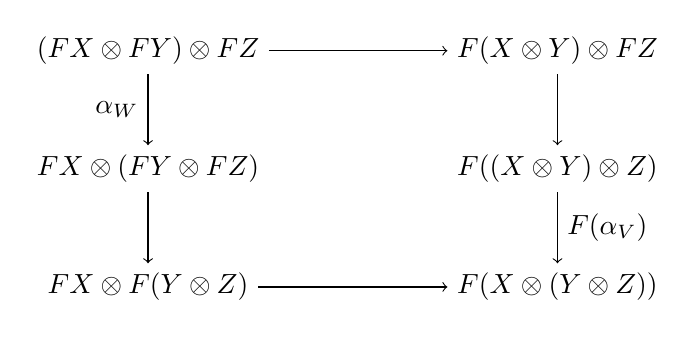
\begin{tikzpicture}
  \node (a) at (0,0) {$(FX \otimes FY) \otimes FZ$};
  \node (b) at (5.2,0) {$F(X \otimes Y) \otimes FZ$};
  \node (c) at (0,-1.5) {$FX \otimes (FY \otimes FZ)$};
  \node (d) at (5.2,-1.5) {$F((X \otimes Y) \otimes Z)$};
  \node (e) at (0,-3) {$FX \otimes F(Y \otimes Z)$};
  \node (f) at (5.2,-3) {$F(X \otimes (Y \otimes Z))$};
  \draw[->] (a) -- (b);
  \draw[->] (a) -- node[left] {$\alpha_W$} (c);
  \draw[->] (b) -- (d);
  \draw[->] (c) -- (e);
  \draw[->] (d) -- node[right] {$F(\alpha_V)$} (f);
  \draw[->] (e) -- (f);
\end{tikzpicture}
\end{center}
其中 $\alpha_W$ 与 $\alpha_V$ 分别是 $(W, \otimes, \mathbf{1})$ 与
$(V, \otimes, \mathbf{1})$ 中的结合同构。对单位亦有同样的要求：
\begin{center}
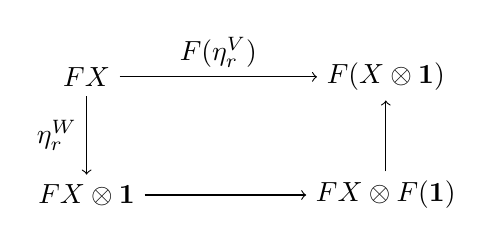
\begin{tikzpicture}
  \node (a) at (0,0) {$FX$};
  \node (b) at (3.8,0) {$F(X \otimes \mathbf{1})$};
  \node (c) at (0,-1.5) {$FX \otimes \mathbf{1}$};
  \node (d) at (3.8,-1.5) {$FX \otimes F(\mathbf{1})$};
  \draw[->] (a) -- node[above] {$F(\eta_r^V)$} (b);
  \draw[->] (a) -- node[left] {$\eta_r^W$} (c);
  \draw[->] (c) -- (d);
  \draw[->] (d) -- (b);
\end{tikzpicture}
\end{center}
其中 $\eta_r^V$ 与 $\eta_r^W$ 分别是 $V$ 与 $W$ 的右单位同构。类似地，涉及左单位的
那个图表也要求交换。如果（2）与（3）中的自然映射都是同构，那么松幺半（或反松幺半）
\trFunctor{}就称为幺半\trFunctor{}。

\begin{definition}\label{def:lax-monoidal-transformation}
设 $F$ 与 $G$ 是幺半范畴 $V$ 与 $W$ 之间的\trLaxMonoidalFunctor{}。一个\trNaturalTransformation{}%
$\tau\colon F \to G$ 称为\emph{松幺半的}（lax monoidal），若对所有的 $X, Y \in V$，
图表
\begin{center}
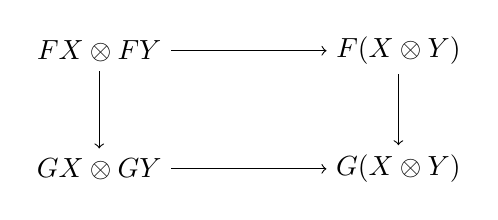
\begin{tikzpicture}
  \node (a) at (0,0) {$FX \otimes FY$};
  \node (b) at (3.8,0) {$F(X \otimes Y)$};
  \node (c) at (0,-1.5) {$GX \otimes GY$};
  \node (d) at (3.8,-1.5) {$G(X \otimes Y)$};
  \draw[->] (a) -- (b);
  \draw[->] (a) -- (c);
  \draw[->] (b) -- (d);
  \draw[->] (c) -- (d);
\end{tikzpicture}
\end{center}
\end{definition}

以及
\begin{center}
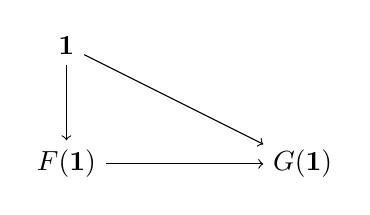
\begin{tikzpicture}
  \node (u) at (0,0) {$\mathbf{1}$};
  \node (f) at (0,-1.5) {$F(\mathbf{1})$};
  \node (g) at (3,-1.5) {$G(\mathbf{1})$};
  \draw[->] (u) -- (f);
  \draw[->] (u) -- (g);
  \draw[->] (f) -- (g);
\end{tikzpicture}
\end{center}
交换。我们记 $\mathrm{Fun}^{\mathrm{lax}}(V, W)$ 为这样的\trCategory{}：其\trObject{}是\trLaxMonoidalFunctor{}，而其\trMorphism{}是松幺半变换。此外，我们记
\[
\mathrm{Fun}^{\otimes}(V, W) \subseteq \mathrm{Fun}^{\mathrm{lax}}(V, W)
\]
为由幺半\trFunctor{}组成的满子范畴。

\begin{remark}\label{rem:moncat-2-category}
于是我们看到，由幺半范畴与幺半\trFunctor{}构成的\trCategory{} $\mathrm{MonCat}$ 典范地是一个
$2$-范畴：$V$ 与 $W$ 之间的 hom-范畴由 $\mathrm{Fun}^{\mathrm{lax}}(V, W)$ 给出。当然，
为了使这一点有意义，我们需要注意到：幺半范畴的恒等\trFunctor{}典范地是松幺半的（事实上是
幺半的），而且两个\trLaxMonoidalFunctor{}的复合典范地是松幺半的。
\end{remark}

\begin{definition}\label{def:v-enriched-category}
设 $(V, \otimes, \mathbf{1})$ 是一个幺半范畴。那么一个 $V$-\trEnrichment{}范畴 $\C$
由一个对象集组成，并且对任意两个对象 $x, y \in \C$ 配有一个对象
$\mathrm{Hom}_{\C}(x, y) \in V$，连同复合\trFunctor{}%
\[
\mathrm{Hom}_{\C}(x, y) \otimes \mathrm{Hom}_{\C}(y, z) \to \mathrm{Hom}_{\C}(x, z),
\]
此外，对每个对象还配有单位 $\mathrm{id}_x$
\[
\mathbf{1} \to \mathrm{Hom}_{\C}(x, x)
\]
满足显然的结合性条件与单位性条件，也就是说，要求下述图表交换：
\begin{center}
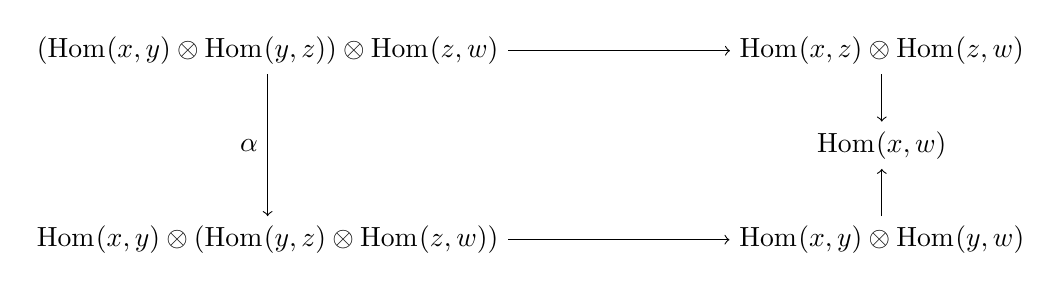
\begin{tikzpicture}
  \node (a) at (0,0) {$(\mathrm{Hom}_{\C}(x, y) \otimes \mathrm{Hom}_{\C}(y, z)) \otimes \mathrm{Hom}_{\C}(z, w)$};
  \node (b) at (7.8,0) {$\mathrm{Hom}_{\C}(x, z) \otimes \mathrm{Hom}_{\C}(z, w)$};
  \node (e) at (7.8,-1.2) {$\mathrm{Hom}_{\C}(x, w)$};
  \node (c) at (0,-2.4) {$\mathrm{Hom}_{\C}(x, y) \otimes (\mathrm{Hom}_{\C}(y, z) \otimes \mathrm{Hom}_{\C}(z, w))$};
  \node (d) at (7.8,-2.4) {$\mathrm{Hom}_{\C}(x, y) \otimes \mathrm{Hom}_{\C}(y, w)$};
  \draw[->] (a) -- (b);
  \draw[->] (a) -- node[left] {$\alpha$} (c);
  \draw[->] (c) -- (d);
  \draw[->] (b) -- (e);
  \draw[->] (d) -- (e);
\end{tikzpicture}
\end{center}
其中 $\alpha$ 表示 $V$ 的结合同构，以及%
\footnote{译注：右侧图表中从左上到右下的斜向箭头在原书中未标注名称；按左图的体例，
应为 $\mathrm{id}$。}
\begin{center}
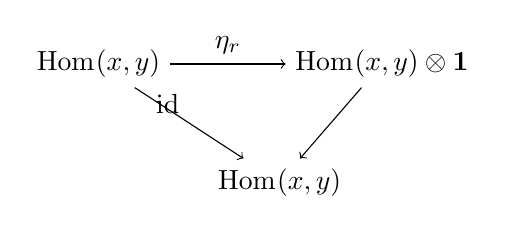
\begin{tikzpicture}
  \node (a) at (0,0) {$\mathrm{Hom}_{\C}(x, y)$};
  \node (b) at (3.6,0) {$\mathrm{Hom}_{\C}(x, y) \otimes \mathbf{1}$};
  \node (c) at (2.3,-1.5) {$\mathrm{Hom}_{\C}(x, y)$};
  \draw[->] (a) -- node[above] {$\eta_r$} (b);
  \draw[->] (a) -- node[above left] {$\mathrm{id}$} (c);
  \draw[->] (b) -- (c);
\end{tikzpicture}
\hspace{2.5em}%
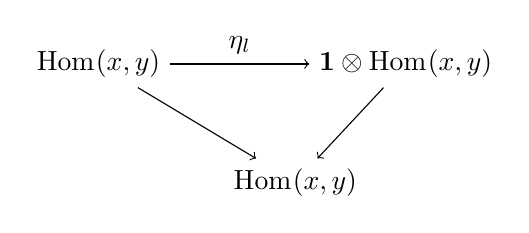
\begin{tikzpicture}
  \node (a) at (0,0) {$\mathrm{Hom}_{\C}(x, y)$};
  \node (b) at (3.9,0) {$\mathbf{1} \otimes \mathrm{Hom}_{\C}(x, y)$};
  \node (c) at (2.5,-1.5) {$\mathrm{Hom}_{\C}(x, y)$};
  \draw[->] (a) -- node[above] {$\eta_l$} (b);
  \draw[->] (a) -- (c);
  \draw[->] (b) -- (c);
\end{tikzpicture}
\end{center}
\end{definition}

\begin{definition}\label{def:v-enriched-functor}
$V$-\trEnrichment{}范畴之间的一个 $V$-\trEnrichment{}\trFunctor{} $f\colon \C \to \D$ 由对象上的
一个映射 $x \mapsto f(x)$ 组成，并且对每两个对象都配有 $V$ 中的一个\trMorphism{}%
$f_{x,y}\colon \mathrm{Hom}_{\C}(x, y) \to \mathrm{Hom}_{\D}(fx, fy)$，使得
图表
\begin{center}
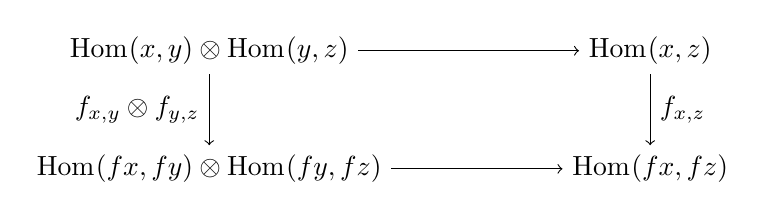
\begin{tikzpicture}
  \node (a) at (0,0) {$\mathrm{Hom}_{\C}(x, y) \otimes \mathrm{Hom}_{\C}(y, z)$};
  \node (b) at (5.6,0) {$\mathrm{Hom}_{\C}(x, z)$};
  \node (c) at (0,-1.5)
    {$\mathrm{Hom}_{\D}(fx, fy) \otimes \mathrm{Hom}_{\D}(fy, fz)$};
  \node (d) at (5.6,-1.5) {$\mathrm{Hom}_{\D}(fx, fz)$};
  \draw[->] (a) -- (b);
  \draw[->] (a) -- node[left] {$f_{x,y} \otimes f_{y,z}$} (c);
  \draw[->] (b) -- node[right] {$f_{x,z}$} (d);
  \draw[->] (c) -- (d);
\end{tikzpicture}
\end{center}
\end{definition}

以及
\begin{center}
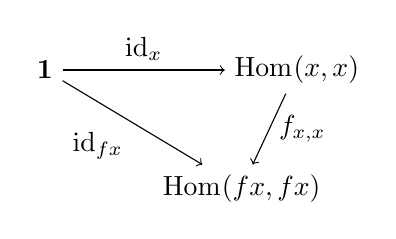
\begin{tikzpicture}
  \node (u) at (0,0) {$\mathbf{1}$};
  \node (a) at (3.2,0) {$\mathrm{Hom}_{\C}(x, x)$};
  \node (b) at (2.5,-1.5) {$\mathrm{Hom}_{\D}(fx, fx)$};
  \draw[->] (u) -- node[above] {$\mathrm{id}_x$} (a);
  \draw[->] (u) -- node[below left] {$\mathrm{id}_{fx}$} (b);
  \draw[->] (a) -- node[right] {$f_{x,x}$} (b);
\end{tikzpicture}
\end{center}
交换。

\begin{definition}\label{def:cat-v}
设 $V$ 是一个幺半范畴。那么我们记 $\mathrm{Cat}_V$ 为 $V$-\trEnrichment{}范畴的\trCategory{}，
也就是说，其\trObject{}是 $V$-\trEnrichment{}范畴，而其\trMorphism{}是 $V$-\trEnrichment{}\trFunctor{}。
\end{definition}

\begin{example*}
一个 $\mathrm{Set}$-\trEnrichment{}范畴恰好就是一个普通\trCategory{}。一个 $\mathrm{Cat}$-\trEnrichment{}%
范畴是一个严格的 $2$-范畴。
\end{example*}

\begin{example*}
一个只有一个对象的 $\mathrm{Cat}$-\trEnrichment{}范畴与一个严格结合的幺半范畴（即其结合同构都
是恒等的幺半范畴）是同一种数据。两个这样的范畴之间的\trEnrichment{}\trFunctor{}与幺半\trFunctor{}也是同一种
数据。
\end{example*}

\begin{lemma}\label{lem:lax-monoidal-cat-v}
设 $\Phi\colon V \to V'$ 是幺半范畴之间的一个\trLaxMonoidalFunctor{}，那么把 $\Phi$ 逐个应用到
每个 hom-对象上便产生一个\trFunctor{} $\Phi_*\colon \mathrm{Cat}_V \to \mathrm{Cat}_{V'}$。事实上，这个构造确定了一个 \trTwoFunctor{}%
\[
\mathrm{MonCat} \to \mathrm{Cat}
\]
它从由幺半范畴构成的 $2$-范畴（以\trLaxMonoidalFunctor{}与幺半变换作为\trMorphism{}与 \trTwoMorphism{}）
映到由\trCategory{}构成的 $2$-范畴（以\trFunctor{}与\trNaturalTransformation{}%
作为\trMorphism{}与 \trTwoMorphism{}）。特别地，$V$ 与 $V'$ 之间的一个\trMonoidalAdjunction{}在\trEnrichment{}范畴的
层面上确定一个\trAdjunction{}。
\end{lemma}

\begin{proof}
为了构造这个 \trTwoFunctor{}，我们首先考虑对象层面上的映射：它把幺半范畴 $V$ 送到 $V$-\trEnrichment{}%
范畴的\trCategory{} $\mathrm{Cat}_V$。为了使这个映射成为一个 \trTwoFunctor{}，我们需要对
每一对幺半范畴 $V$、$W$ 构造一个\trFunctor{}%
\[
\mathrm{Fun}^{\mathrm{lax}}(V, W) \to \mathrm{Fun}(\mathrm{Cat}_V, \mathrm{Cat}_W)
\]
然后再证明这个构造与复合相容。为了构造这个\trFunctor{}，我们还是先考虑它在对象上的
作用：给定\trLaxMonoidalFunctor{} $\Phi\colon V \to W$ 与一个 $V$-\trEnrichment{}范畴 $\C$，我们考虑
$W$-\trEnrichment{}范畴 $\Phi_*(\C)$，其\trObject{}与 $\C$ 的\trObject{}相同，并且对
$X, Y \in \mathrm{ob}(\C)$ 我们定义
\[
\mathrm{Hom}_{\Phi_*(\C)}(X, Y) = \Phi(\mathrm{Hom}_{\C}(X, Y)).
\]
容易验证 $\Phi_*(\C)$ 是一个 $W$-\trEnrichment{}范畴：例如，为了证明复合满足结合性约束，需要
用到 $\Phi$ 与 $V$ 和 $W$ 的结合同构的相容性。接下来，我们需要说明它在\trMorphism{}%
上的作用。为此，设 $\tau\colon \Phi \to \Psi$ 是一个幺半变换。我们希望构造
$\Phi_*$ 与 $\Psi_*$ 之间的一个\trNaturalTransformation{}。具体地说，我们需要在
$\mathrm{Cat}_W$ 中构造自然映射 $\Phi_*(\C) \to \Psi_*(\C)$，也就是说，自然的
$W$-\trEnrichment{}\trFunctor{} $\tau_*\colon \Phi_*(\C) \to \Psi_*(\C)$。在\trObject{}上，这个\trFunctor{}%
定义为恒等，而在 $X$ 与 $Y$ 之间的\trMorphism{}上，我们必须构造一个映射
\[
\tau_*\colon \Phi(\mathrm{Hom}_{\C}(X, Y)) \to \Psi(\mathrm{Hom}_{\C}(X, Y)).
\]
为此，我们只需使用由\trNaturalTransformation{} $\tau\colon \Phi \to \Psi$ 给出的自然
映射 $\tau_{\mathrm{Hom}_{\C}(X, Y)}$。为了看出这与复合相容，我们利用 $\tau$ 是一个
幺半变换这一事实，因而图表
\begin{center}
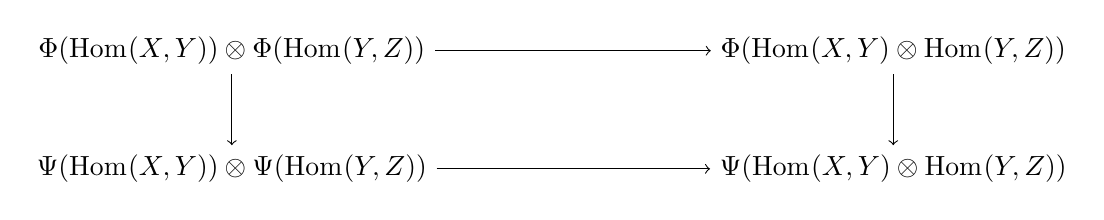
\begin{tikzpicture}
  \node (a) at (0,0)
    {$\Phi(\mathrm{Hom}_{\C}(X, Y)) \otimes \Phi(\mathrm{Hom}_{\C}(Y, Z))$};
  \node (b) at (8.4,0)
    {$\Phi(\mathrm{Hom}_{\C}(X, Y) \otimes \mathrm{Hom}_{\C}(Y, Z))$};
  \node (c) at (0,-1.5)
    {$\Psi(\mathrm{Hom}_{\C}(X, Y)) \otimes \Psi(\mathrm{Hom}_{\C}(Y, Z))$};
  \node (d) at (8.4,-1.5)
    {$\Psi(\mathrm{Hom}_{\C}(X, Y) \otimes \mathrm{Hom}_{\C}(Y, Z))$};
  \draw[->] (a) -- (b);
  \draw[->] (a) -- (c);
  \draw[->] (b) -- (d);
  \draw[->] (c) -- (d);
\end{tikzpicture}
\end{center}
交换。然后用 $\tau$ 的自然性又可看出图表
\begin{center}
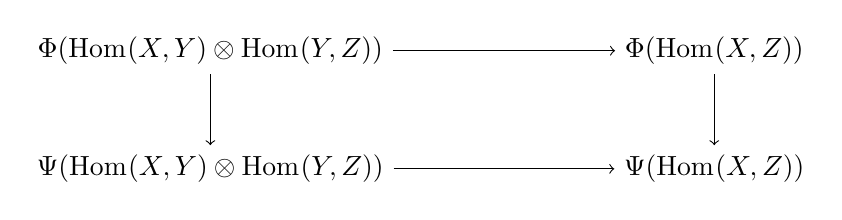
\begin{tikzpicture}
  \node (a) at (0,0)
    {$\Phi(\mathrm{Hom}_{\C}(X, Y) \otimes \mathrm{Hom}_{\C}(Y, Z))$};
  \node (b) at (6.4,0) {$\Phi(\mathrm{Hom}_{\C}(X, Z))$};
  \node (c) at (0,-1.5)
    {$\Psi(\mathrm{Hom}_{\C}(X, Y) \otimes \mathrm{Hom}_{\C}(Y, Z))$};
  \node (d) at (6.4,-1.5) {$\Psi(\mathrm{Hom}_{\C}(X, Z))$};
  \draw[->] (a) -- (b);
  \draw[->] (a) -- (c);
  \draw[->] (b) -- (d);
  \draw[->] (c) -- (d);
\end{tikzpicture}
\end{center}
也交换。把这两个图表拼接起来，我们发现映射 $\tau_*$ 与复合相容，因而正如所需，它事
实上是一个 $W$-\trEnrichment{}\trFunctor{} $\Phi_*(\C) \to \Psi_*(\C)$。

现在，由定义也显然可知：对两个可复合的\trLaxMonoidalFunctor{} $\Psi$ 与 $\Phi$，我们有
$\Psi_*(\Phi_*(\C)) = (\Psi \circ \Phi)_*(\C)$，因此与复合的相容性是眼前的直接
推论。

至于断言中「特别地」的部分，现在容易看出：一个\trMonoidalAdjunction{}由\trLaxMonoidalFunctor{} $\Phi$ 与
$\Psi$ 以及单位与余单位变换组成，而这些变换本身是幺半变换。由前面已建立的部分，
它们被送到配备了单位与余单位候选者的\trFunctor{} $\Phi_*$ 与 $\Psi_*$。唯一需要验证的是
三角形恒等式，但它可以由这些恒等式对 $\Phi$ 与 $\Psi$ 成立、以及所构造的\trFunctor{}保持
恒等这一事实得出。
\end{proof}

\begin{definition}\label{def:underlying-category}
设 $V$ 是一个幺半范畴，$\C$ 是一个 $V$-\trEnrichment{}范畴。那么它的\emph{\trUnderlyingCategory{}}（underlying
category）$u\C$ 经由\trLaxMonoidalFunctor{}%
\[
\mathrm{Hom}(\mathbf{1}, -)\colon V \to \mathrm{Set}
\]
而得到。
\end{definition}

用公式来写，我们有
\[
u\C = \mathrm{Hom}_V(\mathbf{1}, -)_*(\C) \in \mathrm{Cat}_{\mathrm{Set}} = \mathrm{Cat}.
\]

\begin{definition}\label{def:simplicial-category}
为简单起见，我们把\trEnrichment{}于\trSimplicialSets{}中的\trCategory{}称为%
\emph{\trSimplicialCategory{}}（simplicial category）。这里，$\mathrm{sSet}$ 经由
笛卡尔积被看作一个幺半范畴，并且我们将用 $\mathrm{Cat}_{\Delta}$ 来记
$\mathrm{Cat}_{\mathrm{sSet}}$。
\end{definition}

\begin{remark}\label{rem:simplicial-category-ambiguity}
注意，上面的定义有几分含混：通常「\trSimplicialCategory{}」一词更愿意指范畴中的单纯对象，也就是
说，一个\trFunctor{} $\Delta^{\mathrm{op}} \to \mathrm{Cat}$。幸运的是，关于这一点
我们有下述引理：
\end{remark}

\begin{lemma}\label{lem:cat-delta-embedding}
存在一个典范的\trFullyFaithful{}嵌入 $\mathrm{Cat}_{\Delta} \to \mathrm{Fun}(\Delta^{\mathrm{op}}, \mathrm{Cat})$，它由\trFunctor{}族
$(\mathrm{ev}_n)_*\colon \mathrm{Cat}_{\Delta} \to \mathrm{Cat}$ 所确定，而其本质像
可以刻画为那些其对象的底\trSimplicialSet{}为常值的范畴中的单纯对象。
\end{lemma}

\begin{lemma}\label{lem:cocomplete-left-adjoint}
设 $F\colon \C \to \D$ 是 $G\colon \D \to \C$ 的\trLeftAdjoint{}。
此外，设：
\begin{enumerate}[label=(\arabic*)]
  \item $\C$ 是余完备的；并且
  \item $G$ 是\trFullyFaithful{}。
\end{enumerate}
那么 $\D$ 也是余完备的。
对偶地，若 $\D$ 是完备的且 $F$ 是\trFullyFaithful{}，那么 $\C$ 也是完备的。
\end{lemma}

\begin{proof}
设（1）与（2）成立。设 $X\colon I \to \D$ 是一个图表，并考虑对象
$F(\operatorname{colim}_I G(X_i))$，由于 $\C$ 余完备，它存在。我们希望证明它满足%
\trColimit{}的泛性质：
\[
\begin{aligned}
\mathrm{Hom}_{\D}(F(\operatorname{colim}_I G(X_i)), Y)
&\cong \mathrm{Hom}_{\C}(\operatorname{colim}_I G(X_i), G(Y))\\
&\cong \lim_I \mathrm{Hom}_{\C}(G(X_i), G(Y))\\
&\cong \lim_I \mathrm{Hom}_{\C}(X_i, Y)
\end{aligned}
\]
其中最后一个双射由 $G$ 的全忠实性成立。

对偶地，设 $X\colon I \to \C$ 是一个图表，并考虑对象 $G(\lim_I F(X_i))$，由于
$\D$ 完备，它存在。那么我们计算出
\[
\begin{aligned}
\mathrm{Hom}_{\C}(Y, G(\lim_I F(X_i)))
&\cong \mathrm{Hom}_{\D}(F(Y), \lim_I F(X_i))\\
&\cong \lim_I \mathrm{Hom}_{\D}(F(Y), F(X_i))\\
&\cong \lim_I \mathrm{Hom}_{\C}(Y, X_i),
\end{aligned}
\]
其中最后一个双射使用了 $F$ 是\trFullyFaithful{}这一事实。
\end{proof}

\begin{proposition}\label{prop:cat-bicomplete}
\trCategory{} $\mathrm{Cat}$ 是\trBicomplete{}的，而且\trFunctor{}%
$\mathrm{ob}(-)\colon \mathrm{Cat} \to \mathrm{Set}$ 保持\trLimit{}与\trColimit{}。
\end{proposition}

\begin{proof}
极限的情形可以手工完成：给定图表 $\C\colon I \to \mathrm{Cat}$，它把 $i \in I$ 送到
$\C_i$，我们如下定义其\trLimit{} $\lim_I \C_i$：
\begin{enumerate}[label=(\arabic*)]
  \item $\mathrm{ob}(\lim_I \C_i) = \lim_I \mathrm{ob}(\C_i)$；并且
  \item 对任意两个对象 $\{X_i\}_{i \in I}$ 与 $\{Y_i\}_{i \in I}$，我们有
  \[
  \mathrm{Hom}_{\lim_I \C_i}(\{X_i\}, \{Y_i\}) =
  \lim_I \mathrm{Hom}_{\C_i}(X_i, Y_i).
  \]
\end{enumerate}
为了看出这事实上是一个\trCategory{}，我们利用「\trLimit{}与积交换」（在定义复合时）
这一事实，以及「从在 $I \times I$ 上取指标的\trLimit{}到沿对角线限制在 $I$ 上取指标
的\trLimit{}存在典范映射」这一事实。（这正是使余极限的情形更为复杂的原因之一。）
于是按定义，\trFunctor{} $\mathrm{ob}(-)\colon \mathrm{Cat} \to \mathrm{Set}$ 与\trLimit{}%
交换（它也必须如此，因为它是离散范畴\trFunctor{} $d\colon \mathrm{Set} \to \mathrm{Cat}$ 的\trRightAdjoint{}）。

为了证明余极限的存在性，我们利用\cref{lem:cocomplete-left-adjoint}：我们考虑
\cref{prop:h-n-adjoint} 中 $\mathrm{sSet}$ 与 $\mathrm{Cat}$ 之间的\trFunctor{}给出的那个%
\trAdjunction{} $(h, \mathrm{N})$。我们已经看到：
\begin{enumerate}[label=(\arabic*)]
  \item $\mathrm{sSet}$ 是余完备的（事实上，由推论 1.1.24 它还是\trBicomplete{}的）；
  并且
  \item $\mathrm{N}\colon \mathrm{Cat} \to \mathrm{sSet}$ 是\trFullyFaithful{}，见
  \cref{cor:nerve-fully-faithful}。
\end{enumerate}
由此得出 $\mathrm{Cat}$ 是余完备的，而且图表 $\C\colon I \to \mathrm{Cat}$ 的一
个\trColimit{}由 $h(\operatorname{colim}_I \mathrm{N}(\C_i))$ 给出。据此，我们如下
计算对象\trFunctor{}与余极限的交换：
\[
\begin{aligned}
\mathrm{ob}(\operatorname{colim}_I \C_i)
&\cong \mathrm{ob}(h(\operatorname{colim}_I \mathrm{N}(\C_i)))\\
&\cong (\operatorname{colim}_I \mathrm{N}(\C_i))_0
\cong \operatorname{colim}_I (\mathrm{N}(\C_i)_0)\\
&\cong \operatorname{colim}_I \mathrm{ob}(\C_i)
\end{aligned}
\]
\end{proof}

\begin{lemma}\label{lem:full-subcategory-colimit}
设 $\C' \subseteq \C$ 是\trCategory{} $\C$ 的一个满子范畴，并设 $X\colon I \to \C'$
是一个图表。若 $X$ 在 $\C$ 中有一个恰好落在 $\C'$ 内的（余）\trLimit{}，那么它也是
$\C'$ 中的（余）\trLimit{}。
\end{lemma}

\begin{proof}
由泛性质以及包含为满的这一事实，显然。
\end{proof}

\begin{corollary}\label{cor:cat-delta-bicomplete}
\trCategory{} $\mathrm{Cat}_{\Delta}$ 是\trBicomplete{}的。
\end{corollary}

\begin{proof}
考虑\trSimplicialCategory{}的一个 $I$ 形图表 $\C_i$。由%
\cref{lem:cat-delta-embedding}，这给出 $\mathrm{Fun}(\Delta^{\mathrm{op}}, \mathrm{Cat})$ 中的一个 $I$ 形图表，其相伴的对象底\trSimplicialSets{}的 $I$ 形图表是
常值的\footnote{译注：原书此处作「in constant」，疑为「is constant」之误。}，也就是
说，对所有的 $i \in I$，我们发现 $\mathrm{ob}(\C_i)$ 是一个常值%
\trSimplicialSet{}。我们希望证明：此时 $\mathrm{ob}(\operatorname{colim}_I \C_i)$
也是常值\trSimplicialSet{}。由\cref{prop:cat-bicomplete}，我们有
\[
\mathrm{ob}(\operatorname{colim}_I \C_i) \cong
\operatorname{colim}_I \mathrm{ob}(\C_i),
\]
而后者是\trSimplicialSets{}中在常值\trSimplicialSets{}上取的\trColimit{}。由于常值\trFunctor{} $c\colon \mathrm{Set} \to \mathrm{sSet}$ 容许一个\trRightAdjoint{}%
（$\mathrm{ev}_0$），它保持余极限。因此，在常值\trSimplicialSets{}上取的\trColimit{}%
本身是常值的（取在所涉诸集合的\trColimit{}之上）。对极限的论证类似。
\end{proof}

\begin{remark}\label{rem:cat-pc-bicomplete}
这里 $\Delta$ 并没有什么特殊。事实上，同样的论证可以证明：对任何小\trCategory{}%
$\C$，存在一个\trFullyFaithful{}包含
$\mathrm{Cat}_{\mathcal{P}(\C)} \subseteq \mathrm{Fun}(\C^{\mathrm{op}}, \mathrm{Cat})$，
其本质像由那些对象的\trPresheaf{}为常值的\trFunctor{}%
给出。完全类似地可得 $\mathrm{Cat}_{\mathcal{P}(\C)}$ 是\trBicomplete{}的。这里我们
总是使用 $\mathcal{P}(\C)$ 上逐点的（笛卡尔）\trMonoidalStructure{}。
\end{remark}

\begin{example*}
\trNerve{}\trFunctor{} $\mathrm{N}\colon \mathrm{Cat} \to \mathrm{sSet}$ 是幺半的：
由于它是一个\trRightAdjoint{}，它保持积。于是，给定一个 $2$-范畴，把\trNerve{}\trFunctor{}%
应用到所有 hom-范畴上，我们便得到一个\trSimplicialCategory{}。此外，对一个 $2$-范畴
$\C$，我们有 $u(\mathrm{N}_*(\C)) = u\C$，原因很简单：
\[
\begin{aligned}
\mathrm{Hom}_{\mathrm{sSet}}(\Delta^0, -)_* \circ \mathrm{N}_*
&= (\mathrm{Hom}_{\mathrm{sSet}}(\Delta^0, -) \circ \mathrm{N})\\
&= \mathrm{Hom}_{\mathrm{sSet}}(\Delta^0, \mathrm{N}(-))\\
&= \mathrm{Hom}_{\mathrm{Cat}}(h\Delta^0, -),
\end{aligned}
\]
而 $h\Delta^0$ 是 $\mathrm{Cat}$ 上由笛卡尔积给出的\trMonoidalStructure{}的单位。
\end{example*}

\begin{lemma}\label{lem:canonically-monoidal}
\trFunctor{} $c\colon \mathrm{Set} \to \mathrm{sSet}$ 与
$\pi_0$、$\mathrm{ev}_0\colon \mathrm{sSet} \to \mathrm{Set}$ 都是典范幺半的。
\end{lemma}

\begin{proof}
我们断言：每个\trFunctor{} $F\colon (V, \times, *) \to (W, \times, *)$ 都典范地是反松
幺半的。反松幺半结构映射由以下给出：
\begin{enumerate}[label=\arabic*.]
  \item $F(*) \to *$，即到 $W$ 的\trTerminalObject{}的唯一映射；以及
  \item $F(X \times Y) \to F(X) \times F(Y)$，由 $F$ 在两个投射
  \[
  X \leftarrow X \times Y \rightarrow Y
  \]
  上的作用给出。
\end{enumerate}
于是只需验证我们的例子中那些典范的反松结构映射都是同构。对 $c$ 与 $\mathrm{ev}_0$
而言，这直接由定义得出。只有\trFunctor{} $\pi_0$\footnote{译注：即\cref{def:pi0} 中的
$\pi^{\Delta}_0$；原书在此处将其简写作 $\pi_0$。}需要真正的论证。我们想验证映射
\[
\pi_0(X \times Y) \to \pi_0(X) \times \pi_0(Y)
\]
是双射。由\trSimplicialSet{}的 $\pi_0$ 的定义（\cref{def:pi0}），我们有一个交换方形
\begin{center}
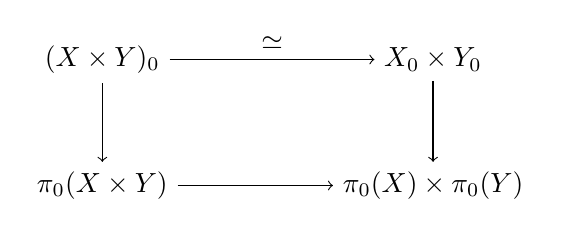
\begin{tikzpicture}
  \node (a) at (0,0) {$(X \times Y)_0$};
  \node (b) at (4.2,0) {$X_0 \times Y_0$};
  \node (c) at (0,-1.6) {$\pi_0(X \times Y)$};
  \node (d) at (4.2,-1.6) {$\pi_0(X) \times \pi_0(Y)$};
  \draw[->] (a) -- node[above] {$\simeq$} (b);
  \draw[->] (a) -- (c);
  \draw[->] (b) -- (d);
  \draw[->] (c) -- (d);
\end{tikzpicture}
\end{center}
其中竖直映射都是双射。由于上面的水平映射是双射（这正是 $\mathrm{ev}_0$ 的幺半性），
反松幺半结构映射是满射。为了看出它是单射，只需验证诸关系的生成元可以被提升。由于
这些生成元由 $1$-\trSimplex{}给出，而 $\mathrm{ev}_1$ 也是幺半的，断言得证。此外，直接可得
映射 $\pi_0(*) \to *$ 是同构。
\end{proof}

\begin{definition}\label{def:functors-cat-delta}
我们得到以下\trFunctor{}：
\begin{enumerate}[label=(\arabic*)]
  \item $c = c_*\colon \mathrm{Cat} \to \mathrm{Cat}_{\Delta}$，它把一个\trCategory{}%
  送到具有常值单纯\trEnrichment{}的那个\trSimplicialCategory{}；
  \item $\pi = (\pi_0)_*\colon \mathrm{Cat}_{\Delta} \to \mathrm{Cat}$，称为%
  \trSimplicialCategory{}的\emph{\trHomotopy{}范畴}；以及
  \item $u = (\mathrm{ev}_0)_*\colon \mathrm{Cat}_{\Delta} \to \mathrm{Cat}$，称为\emph{\trUnderlyingCategory{}}。
\end{enumerate}
注意 $\mathrm{ev}_0 = \mathrm{Hom}_{\mathrm{sSet}}(\Delta^0, -)$，因此它与
\cref{def:underlying-category} 中的\trUnderlyingCategory{}是同一个。
\end{definition}

\begin{definition}\label{def:weak-equivalence-simplicial}
\trSimplicialCategory{}之间的一个单纯\trFunctor{} $f\colon \C \to \D$ 称为一个%
\emph{\trWeakEquivalence{}}（weak equivalence），若它诱导：
\begin{enumerate}[label=(\arabic*)]
  \item 诸 hom-单纯集上的\trWeakEquivalence{}（即它是\trWeaklyFullyFaithful{}）；以及
  \item 一个\trEssentiallySurjective{}\trFunctor{} $\pi(\C) \to \pi(\D)$（即它是\trWeaklyEssentiallySurjective{}）。
\end{enumerate}
\end{definition}

\begin{lemma}\label{lem:oplax-canonical}
笛卡尔幺半范畴之间的每个\trFunctor{}都典范地是反松幺半的。两个这样的\trFunctor{}之间的每个\trNaturalTransformation{}%
也是典范地反松幺半的。特别地，\trAdjunction{}对 $(\pi_0, c)$ 与
$(c, \mathrm{ev}_0)$ 是\trMonoidalAdjunction{}。
\end{lemma}

\begin{proof}
在\cref{lem:canonically-monoidal} 的证明中我们已经看到，每个\trFunctor{}%
$F\colon (V, \times, *) \to (W, \times, *)$ 都典范地是反松幺半的。设
$\tau\colon F \to G$ 是一个\trNaturalTransformation{}。我们希望证明图表
\begin{center}
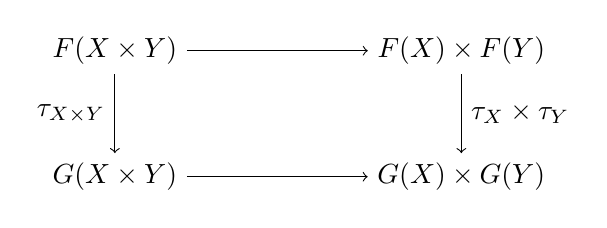
\begin{tikzpicture}
  \node (a) at (0,0) {$F(X \times Y)$};
  \node (b) at (4.4,0) {$F(X) \times F(Y)$};
  \node (c) at (0,-1.6) {$G(X \times Y)$};
  \node (d) at (4.4,-1.6) {$G(X) \times G(Y)$};
  \draw[->] (a) -- (b);
  \draw[->] (a) -- node[left] {$\tau_{X \times Y}$} (c);
  \draw[->] (b) -- node[right] {$\tau_X \times \tau_Y$} (d);
  \draw[->] (c) -- (d);
\end{tikzpicture}
\end{center}
交换。为此，只需验证下面两个方形中的每一个都交换：
\begin{center}
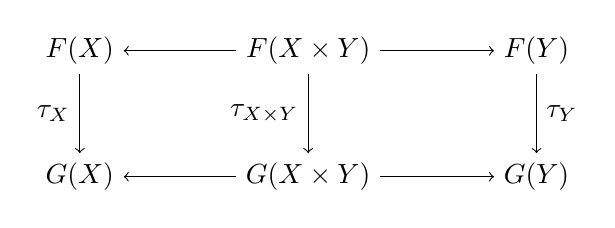
\begin{tikzpicture}
  \node (a) at (0,0) {$F(X)$};
  \node (b) at (2.9,0) {$F(X \times Y)$};
  \node (c) at (5.8,0) {$F(Y)$};
  \node (d) at (0,-1.6) {$G(X)$};
  \node (e) at (2.9,-1.6) {$G(X \times Y)$};
  \node (f) at (5.8,-1.6) {$G(Y)$};
  \draw[->] (b) -- (a);
  \draw[->] (b) -- (c);
  \draw[->] (a) -- node[left] {$\tau_X$} (d);
  \draw[->] (b) -- node[left] {$\tau_{X \times Y}$} (e);
  \draw[->] (c) -- node[right] {$\tau_Y$} (f);
  \draw[->] (e) -- (d);
  \draw[->] (e) -- (f);
\end{tikzpicture}
\end{center}
但这可以由 $\tau$ 的自然性得出。

现在只需证明：幺半\trFunctor{}之间的一个反松幺半变换也是幺半变换。而这可以由下述一般事实
得出\footnote{译注：原书此句作「if a square which both vertical maps being
isomorphisms commutes」，文法有脱漏，疑为「if a square with both vertical maps
being isomorphisms commutes」，兹按其意译出。}：若一个两个竖直映射都是同构的方形
交换，那么把竖直映射换成其逆之后的方形也交换。
\end{proof}

\begin{corollary}\label{cor:adjoint-pairs-cat-delta}
两个\trFunctor{} $c\colon \mathrm{Cat} \to \mathrm{Cat}_{\Delta}$ 与
$\pi\colon \mathrm{Cat}_{\Delta} \to \mathrm{Cat}$ 构成一个\trAdjunction{}对，其中 $\pi$ 是常值\trFunctor{} $c$ 的\trLeftAdjoint{}。类似地，两个\trFunctor{}%
$u\colon \mathrm{Cat}_{\Delta} \to \mathrm{Cat}$ 与
$c\colon \mathrm{Cat} \to \mathrm{Cat}_{\Delta}$ 构成一个\trAdjunction{}对，其中 $c$ 是底\trFunctor{}的\trLeftAdjoint{}。
\end{corollary}

\begin{proof}
这由\cref{lem:lax-monoidal-cat-v} 与\cref{lem:oplax-canonical} 得出。
\end{proof}

\begin{observation}\label{obs:canonical-functor-c-pi}
该\trAdjunction{}产生了\trSimplicialCategory{}的一个典范\trFunctor{} $\C \to c\pi(\C)$。
\end{observation}

\begin{definition}\label{def:morphism-simplicial-category}
给定一个\trSimplicialCategory{} $\C$ 与两个对象 $x, y \in \C$，我们说从 $x$ 到 $y$
的一个\trMorphism{}是指\trUnderlyingCategory{} $u\C$ 中的一个\trMorphism{}。换言之，它是
$\mathrm{Hom}_{\C}(x, y)$ 的一个 $0$-\trSimplex{}。这样一个\trMorphism{}称为一个%
\emph{\trEquivalence{}}（equivalence），若它在 $\pi(\C)$ 中的像是同构。
\end{definition}

接下来，我们希望把\trCategory{}的\trNerve{}这一概念推广到单纯\trEnrichment{}范畴。为此，我们
需要\trCategory{} $[n]$ 的一个适合单纯\trEnrichment{}范畴的版本。

\begin{definition}\label{def:p-i-j}
设 $J$ 是一个非空的有限线性序集，并设 $i$、$j$ 是这个集合的元素。我们令 $P_{i,j}$ 为
$J$ 的下述子集之集：
\[
P_{i,j} = \{\, I \subseteq J : i, j \in I \text{ 并且 } k \in I \Rightarrow
i \le k \le j \,\}
\]
用文字来说，$P_{i,j}$ 由 $[i, j] \subseteq J$ 的所有包含 $i$ 与 $j$ 的子集组成。
$P_{i,j}$ 按包含关系成为偏序集：$I \le I' \iff I \subseteq I'$。注意，仅当
$i \le j$ 时 $P_{i,j}$ 才非空。
\end{definition}

\begin{observation}\label{obs:p-i-j-union}
给定 $J$ 中的一个三元组 $i \le j \le k$，存在偏序集的一个典范映射
\[
P_{i,j} \times P_{j,k} \to P_{i,k},
\]
它由把 $(I, I')$ 送到 $I \cup I'$ 给出。这显然定义了一个结合的二元运算。
\end{observation}

作为推论，我们得到下述定义。

\begin{definition}\label{def:c-delta-j}
设 $J$ 是一个非空的线性序集。那么下述数据定义了一个单纯\trEnrichment{}范畴
$\mathfrak{C}[\Delta^J] \in \mathrm{Cat}_{\Delta}$。
$\mathfrak{C}[\Delta^J]$ 的\trObject{}由 $J$ 的元素给出。此外，
\[
\mathrm{Hom}_{\mathfrak{C}[\Delta^J]}(i, j) =
\begin{cases}
\varnothing & \text{若 } j < i,\\
\mathrm{N}(P_{i,j}) & \text{若 } i \le j.
\end{cases}
\]
\end{definition}

复合经由前一个观察来定义。

\begin{lemma}\label{lem:nerve-p-0-n}
对每个 $n \ge 1$，我们有 $\mathrm{N}(P_{0,n})$ 同构于 $(\Delta^1)^{n-1}$。此外，
$P_{i,j} \cong P_{0,j-i}$。
\end{lemma}

\begin{proof}
后一个陈述只需选取某个同构 $J \cong [n]$（对某个 $n$），然后考虑 $[i, j]$ 与
$[0, j-i]$ 之间唯一的保序同构即可。为了证明
$\mathrm{N}(P_{0,n}) \cong (\Delta^1)^{n-1}$，只需找到一个偏序集的同构
\[
P_{0,n} \cong [1] \times \dotsb \times [1],
\]
其中右边的乘积有 $n-1$ 个因子。这直接来自下述构造：包含 $\{0, n\}$ 的子集
$I \subseteq [n]$ 由检查 $1, \dots, n-1$ 中哪些元素含于 $I$ 而确定。我们把含于 $I$
的元素标为 $1$，把不含于 $I$ 的元素标为 $0$。这就构造出偏序集的一个映射
$P_{0,n} \to [1] \times \dotsb \times [1]$，它显然是一个同构。
\end{proof}

\begin{lemma}\label{lem:nerve-initial-terminal-contractible}
设 $\C$ 是一个有\trInitialObject{}或\trTerminalObject{}的\trCategory{}。那么
$\mathrm{N}(\C)$ 是可缩的，也就是说，它的恒等映射\trHomotopy{}于在\trInitialObject{}或%
\trTerminalObject{}处的常值映射。
\end{lemma}

\begin{proof}
让我们考虑 $\C$ 有\trInitialObject{} $\varnothing$ 的情形。（另一种情形由「\trSimplicialSet{}%
$X$ 可缩当且仅当 $X^{\mathrm{op}}$ 可缩」这一事实得出。）我们断言：$\C$ 的恒等\trFunctor{}%
容许一个从取值为 $\varnothing$ 的常值\trFunctor{}出发的\trNaturalTransformation{}，它在对象
$X \in \C$ 上简单地由唯一映射 $\varnothing \to X$ 给出。相关的图表由这些映射的唯一
性而交换。我们得到一个\trFunctor{} $\C \times [1] \to \C$，它在 $0$ 上的限制是 $\varnothing$
处的常值映射，而在 $1$ 上的限制是 $\C$ 的恒等。应用\trNerve{}\trFunctor{} $\mathrm{N}$，我们
得到一个单纯\trHomotopy{}%
\[
\mathrm{N}(\C) \times \Delta^1 \to \mathrm{N}(\C)
\]
它从由 $\varnothing$ 给出的顶点处的常值映射到 $\mathrm{N}(\C)$ 的恒等。
\end{proof}

\begin{corollary}\label{cor:hom-c-delta-j-contractible}
对 $i \le j$，\trSimplicialSet{} $\mathrm{Hom}_{\mathfrak{C}[\Delta^J]}(i, j)$ 是可缩的。
\end{corollary}

\begin{proof}
我们刚刚看到
$\mathrm{Hom}_{\mathfrak{C}[\Delta^J]}(i, j) \cong \Delta^{j-i-1} = \mathrm{N}([1] \times \dotsb \times [1])$。
范畴 $[1] \times \dotsb \times [1]$ 既有\trInitialObject{}又有\trTerminalObject{}，
于是可以应用\cref{lem:nerve-initial-terminal-contractible}。
\end{proof}

\begin{remark}\label{rem:realization-preserves-products}
\trFunctor{} $|-|\colon \mathrm{sSet} \to \mathrm{Top}$ 保持积。为了看出这一点，只需验证
$|\Delta^n \times \Delta^m| \cong |\Delta^n|_{\mathrm{top}} \times |\Delta^m|_{\mathrm{top}}$，
这是一个具体的计算。因此，单纯\trHomotopy{}诱导\trGeometricRealization{}的\trHomotopy{}。
由此得出：每个可缩的\trSimplicialSet{}都是弱可缩的（即其\trGeometricRealization{}是可缩的）。
\end{remark}

\begin{lemma}\label{lem:pi-c-delta-n}
存在唯一的在对象上为恒等的同构 $\pi(\mathfrak{C}[\Delta^n]) \cong [n]$。经由\trAdjunction{}，
我们得到一个典范\trFunctor{} $\mathfrak{C}[\Delta^n] \to c[n]$，而这个\trFunctor{}是\trSimplicialCategory{}的一个\trWeakEquivalence{}。
\end{lemma}

\begin{proof}
一切都由\cref{cor:hom-c-delta-j-contractible} 得出，后者把
$\pi(\mathfrak{C}[\Delta^n])$ 计算为 $[n]$。由此，诱导\trFunctor{}%
$\mathfrak{C}[\Delta^n] \to c[n]$ 在对象上是双射的（因而\trWeaklyEssentiallySurjective{}），并且在
hom-单纯集上是\trWeakEquivalence{}。
\end{proof}

\begin{lemma}\label{lem:c-delta-j-functor}
结合 $J \mapsto \mathfrak{C}[\Delta^J]$ 可扩充成一个\trFunctor{}%
\[
\mathrm{LinOrdSet} \to \mathrm{Cat}_{\Delta}.
\]
特别地，我们得到一个\trFunctor{}%
\[
\Delta \to \mathrm{Cat}_{\Delta} \qquad [n] \mapsto \mathfrak{C}[\Delta^n]
\]
它是单纯\trEnrichment{}范畴中的一个\trCosimplicial{}对象。
\end{lemma}

\begin{proof}
我们需要证明：线性序集之间的每个映射 $J \to J'$ 都诱导一个单纯\trEnrichment{}\trFunctor{}%
$\mathfrak{C}[\Delta^J] \to \mathfrak{C}[\Delta^{J'}]$。为此，只需解释这样的映射
$J \to J'$ 如何对 $J$ 中每一对 $i \le j$ 诱导偏序集的一个映射
$P_{i,j} \to P_{f(i), f(j)}$。这个映射简单地由把子集 $I$ 送到它的像 $f(I)$ 给出。容易
看出，这事实上产生一个\trFunctor{}。
\end{proof}

\begin{definition}\label{def:simplicial-nerve}
设 $\C$ 是一个单纯\trEnrichment{}范畴。那么我们把它\emph{单纯\trNerve{}}（simplicial nerve）
（或\trCoherentNerve{}，homotopy-coherent nerve）定义为如下\trSimplicialSet{}：
\[
\mathrm{N}(\C)_n = \mathrm{Hom}_{\mathrm{Cat}_{\Delta}}(\mathfrak{C}[\Delta^n], \C)
\]
\end{definition}

\begin{lemma}\label{lem:nerve-c-c}
若 $\C$ 是一个普通\trCategory{}，经由常值\trFunctor{}把它看作单纯\trEnrichment{}范畴 $c\C$，那么存在
同构
\[
\mathrm{N}(\C) \cong \mathrm{N}(c\C).
\]
\end{lemma}

\begin{proof}
这由下式得出：
\[
\begin{aligned}
\mathrm{N}(c\C)_n
&= \mathrm{Hom}_{\mathrm{Cat}_{\Delta}}(\mathfrak{C}[\Delta^n], c\C)\\
&\cong \mathrm{Hom}_{\mathrm{Cat}}(\pi(\mathfrak{C}[\Delta^n]), \C)\\
&\cong \mathrm{Hom}_{\mathrm{Cat}}([n], \C) = \mathrm{N}(\C)_n
\end{aligned}
\]
唯一还需要进一步论证的是同构 $\pi(\mathfrak{C}[\Delta^n]) \cong [n]$，它在
\cref{lem:pi-c-delta-n} 中已得到证明。
\end{proof}

\begin{remark}\label{rem:pi-u-analog-wrong}
把这样的陈述换成用 $\pi(\C)$ 与 $u\C$ 来陈述的类似命题是不成立的！
\end{remark}

\begin{observation}\label{obs:simplicial-nerve-detail}
设 $\C$ 是一个单纯\trEnrichment{}范畴。让我们现在更仔细地考察\trSimplicialSet{} $\mathrm{N}(\C)$。为此，
我们回忆
\[
\mathrm{N}(\C)_n = \mathrm{Hom}_{\mathrm{Cat}_{\Delta}}(\mathfrak{C}[\Delta^n], \C).
\]
展开\trSimplicialCategory{} $\mathfrak{C}[\Delta^0]$ 与 $\mathfrak{C}[\Delta^1]$，我们发现：
\begin{enumerate}[label=(\arabic*)]
  \item $\mathfrak{C}[\Delta^0]$ 是一个只有一个对象的\trSimplicialCategory{}，其
  态射-单纯集由 $\mathrm{N}(P_{0,0})$ 给出，而后者也由 $\Delta^0$ 给出；
  \item $\mathfrak{C}[\Delta^1]$ 是一个有两个对象 $0$ 与 $1$ 的%
  \trSimplicialCategory{}，而且所有态射-单纯集都由 $\Delta^0$ 给出。
\end{enumerate}

换言之，$\mathfrak{C}[\Delta^0]$ 与 $\mathfrak{C}[\Delta^1]$ 分别由 $c[0]$ 与 $c[1]$
给出，这里我们把 $[0]$ 与 $[1]$ 视为\trCategory{}，然后应用常值\trFunctor{}%
$c\colon \mathrm{Cat} \to \mathrm{Cat}_{\Delta}$。作为推论，我们由%
\cref{cor:adjoint-pairs-cat-delta} 得到：
\begin{enumerate}[label=(\arabic*)]
  \item $\mathrm{N}(\C)_0 = \mathrm{Hom}_{\mathrm{Cat}_{\Delta}} (\mathfrak{C}[\Delta^0], \C) \cong \mathrm{Hom}_{\mathrm{Cat}}([0], u\C)$；以及
  \item $\mathrm{N}(\C)_1 = \mathrm{Hom}_{\mathrm{Cat}_{\Delta}} (\mathfrak{C}[\Delta^1], \C) \cong \mathrm{Hom}_{\mathrm{Cat}}([1], u\C)$，
\end{enumerate}
用文字来说，$\mathrm{N}(\C)$ 的\trObject{}由 $\C$ 的\trObject{}给出，而
$\mathrm{N}(\C)$ 的\trMorphism{}由 $\C$ 的\trMorphism{}（即 hom-单纯集的 $0$-\trSimplex{}）
给出。

让我们更进一步，分析\trSimplicialCategory{} $\mathfrak{C}[\Delta^2]$，其\trObject{}由
$\{0, 1, 2\}$ 给出。所有自同态-单纯集都由 $\Delta^0$ 给出。此外，
\[
\mathrm{Hom}_{\mathfrak{C}[\Delta^2]}(0, 1) = \Delta^0 =
\mathrm{Hom}_{\mathfrak{C}[\Delta^2]}(1, 2).
\]
然而，为了分析从 $0$ 到 $2$ 的 hom-单纯集，我们必须考察 $\mathrm{N}(P_{0,2})$。按
定义，$P_{0,2}$ 是 $\{0 < 1 < 2\}$ 的包含 $0$ 与 $2$ 的子集所构成的偏序集。恰好有
两个这样的子集，于是我们得到 $P_{0,2} = [1]$。特别地，
\[
\mathrm{Hom}_{\mathfrak{C}[\Delta^2]}(0, 2) = \mathrm{N}(P_{0,2}) = \Delta^1.
\]

于是我们发现，$\mathrm{N}(\C)$ 中的一个 $2$-\trSimplex{}由以下数据组成：对象 $X$、$Y$ 与 $Z$
（与三个对象 $0$、$1$、$2$ 相关联）；一个\trMorphism{} $f\colon X \to Y$（与
$\mathfrak{C}[\Delta^2]$ 中那个从 $0$ 到 $1$ 的唯一\trMorphism{}相关联）以及一个%
\trMorphism{} $g\colon Y \to Z$（与 $\mathfrak{C}[\Delta^2]$ 中那个从 $1$ 到 $2$ 的
唯一\trMorphism{}相关联）；还有一个 $1$-\trSimplex{} $\Delta^1 \to \mathrm{Hom}_{\C}(X, Z)$
（与 $\mathfrak{C}[\Delta^2]$ 中 $0$ 与 $2$ 之间的 hom-单纯集相关联），其在 $0$ 上的
限制由 $gf$ 给出，而在 $1$ 上的限制由某个别的\trMorphism{}给出。

非正式地说，一个 $2$-\trSimplex{}于是由下面这组数据组成：两个可合成的\trMorphism{}%
$X \to Y$ 与 $Y \to Z$、另一个\trMorphism{} $X \to Z$、以及一个从前两个\trMorphism{}%
的复合到最后那个\trMorphism{}的\trHomotopy{}。
\end{observation}

\begin{lemma}\label{lem:cat-delta-small-colimits}
单纯\trEnrichment{}范畴的\trCategory{} $\mathrm{Cat}_{\Delta}$ 容许所有小的余极限。因此，存在
唯一的一个保持余极限的\trFunctor{}%
\[
\mathfrak{C}[-]\colon \mathrm{sSet} \to \mathrm{Cat}_{\Delta}
\]
它把 $\Delta^n$ 送到 $\mathfrak{C}[\Delta^n]$。这个\trFunctor{}自动地是单纯\trNerve{}\trFunctor{}的\trLeftAdjoint{}。
\end{lemma}

\begin{proof}
余极限的存在性在\cref{cor:cat-delta-bicomplete} 中已经处理。证明的其余部分是形式性
的，而且我们已经多次见过这个论证。
\end{proof}

\begin{fact}\label{fact:c-generated-subcategory}
给定一个\trSimplicialSet{} $X$，考虑子单纯集 $A_i \subseteq X$。那么并集
$A = \bigcup A_i$ 也是 $X$ 的一个子单纯集。在这种情形，我们发现 $\mathfrak{C}[A]$ 是
由诸 $\mathfrak{C}[A_i]$ 生成的 $\mathfrak{C}[X]$ 的子\trSimplicialCategory{}。回忆：\trSimplicialCategory{} $\C$
的一个子\trSimplicialCategory{}由一个对象子集以及——对任意两个这样的对象——$\C$ 中 hom-单纯集的
一个子单纯集所确定。

这个事实例如在 \cite[Corollary 1.15]{Joy07} 中有证明。它根本上依赖于这一事实：\trFunctor{}%
$\mathfrak{C}[-]\colon \mathrm{sSet} \to \mathrm{Cat}_{\Delta}$ 把\trSimplicialSet{}的\trMonomorphism{}送到\trSimplicialCategory{}的\trMonomorphism{}。
\end{fact}

\begin{lemma}\label{lem:c-lambda-n-j}
设 $0 < j < n$ 并考虑\trHorn{} $\Lambda^n_j$。我们有：$\mathfrak{C}[\Lambda^n_j]$
是 $\mathfrak{C}[\Delta^n]$ 的一个子\trSimplicialCategory{}，具有如下性质：
\begin{enumerate}[label=(\arabic*)]
  \item $\mathfrak{C}[\Lambda^n_j]$ 的\trObject{}由 $\Lambda^n_j$ 的顶点给出，因而
  由 $\mathfrak{C}[\Delta^n]$ 的所有对象给出；
  \item hom-单纯集给出如下：
  \[
  \mathrm{Hom}_{\mathfrak{C}[\Lambda^n_j]}(i, k) =
  \mathrm{Hom}_{\mathfrak{C}[\Delta^n]}(i, k)
  \]
  除非 $(i, k) = (0, n)$，并且
  \[
  \mathrm{Hom}_{\mathfrak{C}[\Lambda^n_j]}(0, n) \subseteq
  \mathrm{Hom}_{\mathfrak{C}[\Delta^n]}(0, n) = \mathrm{N}(P_{0,n})
  \]
  由删去内部与底部 $j$-面所得到的 $(\Delta^1)^{n-1}$ 的子单纯集给出。
\end{enumerate}
\end{lemma}

\begin{proof}
让我们首先证明 $\mathfrak{C}[\Lambda^n_j]$ 的这个候选者事实上是
$\mathfrak{C}[\Delta^n]$ 的一个子\trSimplicialCategory{}。我们知道
$\Lambda^n_j = \bigcup_{i \ne j} \Delta^{[n]\setminus\{i\}}$。那么让我们先描述子单纯
范畴
\[
\mathfrak{C}[\Delta^{[n]\setminus\{i\}}] \subseteq \mathfrak{C}[\Delta^n].
\]
这个子范畴的对象由除对应于 $i \in [n]$ 的那个对象之外的所有对象给出。现在设
$k, l \in [n]\setminus\{i\}$，$k \le l$。若 $l < i$，那么存在一个显然的同构
\[
P^{[n]\setminus\{i\}}_{k,l} \cong P^{[n]}_{k,l}
\]
其中上标指明在哪个线性序集中施行\cref{def:p-i-j} 的构造 $P_{k,l}$。于是我们得到
hom-单纯集的一个等式
\[
\mathrm{Hom}_{\mathfrak{C}[\Delta^{[n]\setminus\{i\}}]}(k, l) =
\mathrm{Hom}_{\mathfrak{C}[\Delta^n]}(k, l).
\]
类似地，对 $k > i$ 也存在这样的同构。现在设 $(k, l) \ne (0, n)$，也就是说，$k \ne 0$
或者 $l \ne n$。先设 $k \ne 0$。那么我们有\trSimplicialSet{}的如下包含链：
\[
\mathrm{Hom}_{\mathfrak{C}[\Delta^{[n]\setminus\{0\}}]}(k, l) \subseteq
\mathrm{Hom}_{\mathfrak{C}[\Lambda^n_j]}(k, l) \subseteq
\mathrm{Hom}_{\mathfrak{C}[\Delta^n]}(k, l)
\]
其中由前述论证，其复合是一个等式。因此我们发现，两个包含实际上都必须是等式。若
$l \ne n$，同样的论证可行。总结起来，我们发现
\[
\mathrm{Hom}_{\mathfrak{C}[\Lambda^n_j]}(k, l) =
\mathrm{Hom}_{\mathfrak{C}[\Delta^n]}(k, l)
\]
除非 $(k, l) = (0, n)$。

接下来，让我们确定 $\mathrm{Hom}_{\mathfrak{C}[\Lambda^n_j]}(0, n)$。由%
\cref{fact:c-generated-subcategory}，对每个 $i \ne j$ 且 $i \ne 0, n$，我们有如下
包含：
\[
\mathrm{Hom}_{\mathfrak{C}[\Delta^{[n]\setminus\{i\}}]}(0, n) \subseteq
\mathrm{Hom}_{\mathfrak{C}[\Lambda^n_j]}(0, n) \subseteq
\mathrm{Hom}_{\mathfrak{C}[\Delta^n]}(0, n).
\]
对 $0 < i < n$，我们发现
\[
P^{[n]\setminus\{i\}}_{0,n} \subseteq P^{[n]}_{0,n}
\]
是一个子偏序集，它恰好由那些满足 $i \notin I$ 的 $I \in P^{[n]}_{k,l}$ 组成%
\footnote{译注：原书此处下标印作 $P^{[n]}_{k,l}$，按上下文疑为 $P^{[n]}_{0,n}$ 之误。}。
换言之，它由偏序集的映射
\[
[1]^{\times(n-2)} \to [1]^{\times(n-1)}
\]
给出，后者把一个 $0$ 放到 $[1]^{\times(n-1)}$ 的第 $i$ 个位置上。取\trNerve{}之后，
这就产生映射 $(\Delta^1)^{n-2} \subseteq (\Delta^1)^{n-1}$，它是在第 $i$ 个坐标处取
$\Delta^1$ 的零顶点。由此得出：对每个 $i \ne j$，第 $i$ 个位置取 $0$ 的那个面
$(\Delta^1)^{n-2} \subseteq (\Delta^1)^{n-1}$ 都包含在
$\mathrm{Hom}_{\mathfrak{C}[\Lambda^n_j]}(0, n)$ 之中。我们把第 $i$ 个位置取 $0$ 的
那个面称为\emph{底 $i$-面}。于是我们发现，先验地，底 $j$-面并不包含在
$\mathrm{Hom}_{\mathfrak{C}[\Lambda^n_j]}(0, n)$ 之中，正如引理的陈述所允诺的那样。
剩下要证明的是：顶 $k$-面包含在 $\mathrm{Hom}_{\mathfrak{C}[\Lambda^n_j]}(0, n)$ 之
中（对所有 $0 < k < n$）。为此，我们考虑图表
\begin{center}
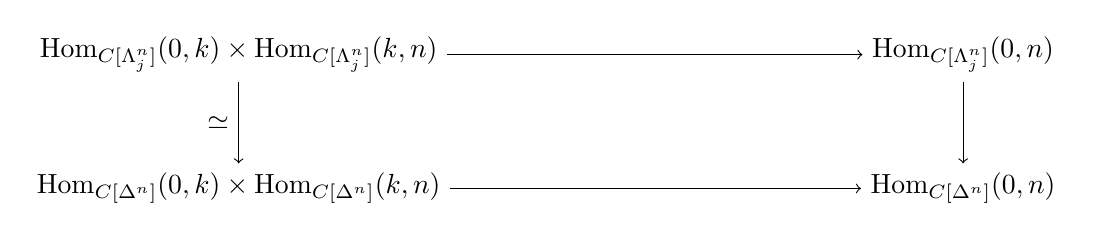
\begin{tikzpicture}
  \node (a) at (0,0) {$\mathrm{Hom}_{\mathfrak{C}[\Lambda^n_j]}(0, k) \times \mathrm{Hom}_{\mathfrak{C}[\Lambda^n_j]}(k, n)$};
  \node (b) at (9.2,0) {$\mathrm{Hom}_{\mathfrak{C}[\Lambda^n_j]}(0, n)$};
  \node (c) at (0,-1.7) {$\mathrm{Hom}_{\mathfrak{C}[\Delta^n]}(0, k) \times \mathrm{Hom}_{\mathfrak{C}[\Delta^n]}(k, n)$};
  \node (d) at (9.2,-1.7) {$\mathrm{Hom}_{\mathfrak{C}[\Delta^n]}(0, n)$};
  \draw[->] (a) -- (b);
  \draw[->] (a) -- node[left] {$\simeq$} (c);
  \draw[->] (b) -- (d);
  \draw[->] (c) -- (d);
\end{tikzpicture}
\end{center}
它编码了相应范畴中的复合。这个图表必须交换，因为
$\mathfrak{C}[\Lambda^n_j]$ 是 $\mathfrak{C}[\Delta^n]$ 的一个子\trSimplicialCategory{}。由于左边
的竖直映射是同构，因此只需证明顶 $i$-面包含在下面那个水平映射的像之中。这个映射由
偏序集的映射
\[
P_{0,k} \times P_{k,n} \to P_{0,n}
\]
诱导，而后者由把 $(I, I')$ 送到 $I \cup I'$ 诱导。由于 $I$ 与 $I'$ 都包含元素 $k$，
在像\cref{lem:nerve-p-0-n} 中那样把这些偏序集等同于立方体之后，我们得到映射
\[
(\Delta^1)^{n-2} \cong (\Delta^1)^{k-1} \times (\Delta^1)^{n-k-1} \to
(\Delta^1)^{n-1}
\]
它由在第 $k$ 个槽位插入一个 $1$ 诱导。这表明顶 $k$-面包含在
$\mathrm{Hom}_{\mathfrak{C}[\Lambda^n_j]}(0, n)$ 之中。由于我们已经知道这个\trPuncturedCube{}产生一个子\trSimplicialCategory{}，而且 $\mathfrak{C}[\Lambda^n_j]$ 包含于其中、并且它自身包含由
$\Delta^n$ 的那些 $i$-面（$i \ne j$）确定的子\trSimplicialCategory{}，引理得证。
\end{proof}

\begin{lemma}\label{lem:coherent-nerve-composer}
\trSimplicialCategory{} $\C$ 的\trCoherentNerve{}是一个\trComposer{}。此外，若所有 hom-单纯集都是%
\trKanComplex{}，也就是说，若它事实上\trEnrichment{}于由\trKanComplex{}构成的对称幺半范畴之
中，那么它是一个\trInfinityCategory{}。
\end{lemma}

\begin{proof}
我们考虑扩张问题
\begin{center}
\begin{tikzpicture}
  \node (a) at (0,0) {$I^n$};
  \node (b) at (3.4,0) {$\mathrm{N}(\C)$};
  \node (c) at (0,-1.5) {$\Delta^n$};
  \draw[->] (a) -- (b);
  \draw[->] (a) -- (c);
  \draw[->, dashed] (c) -- (b);
\end{tikzpicture}
\end{center}
由\trAdjunction{}性，它等价于扩张问题
\begin{center}
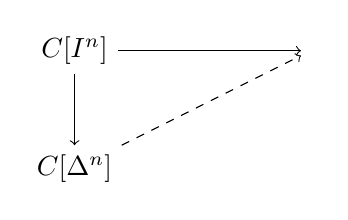
\begin{tikzpicture}
  \node (a) at (0,0) {$\mathfrak{C}[I^n]$};
  \node (b) at (3,0) {$\C$};
  \node (c) at (0,-1.5) {$\mathfrak{C}[\Delta^n]$};
  \draw[->] (a) -- (b);
  \draw[->] (a) -- (c);
  \draw[->, dashed] (c) -- (b);
\end{tikzpicture}
\end{center}
为了证明后者可解，只需证明映射 $\mathfrak{C}[I^n] \to \mathfrak{C}[\Delta^n]$ 有一个
收缩。为了看出这一点，我们首先断言 $\mathfrak{C}[I^n] \cong c[n]$。这可以简单地由
「它对 $n = 1$ 成立」以及随后的归纳得出（利用 $I^n \cong I^{n-1} \amalg_{\Delta^0} I^1$
这一事实以及\trFunctor{} $c\colon \mathrm{Cat} \to \mathrm{Cat}_{\Delta}$ 保持余极限这一事实）。在\cref{lem:pi-c-delta-n} 中我们已经看到，存在唯一的在对象上为恒等的单纯\trFunctor{}%
$\mathfrak{C}[\Delta^n] \to c[n]$。于是，复合
\[
c[n] \cong \mathfrak{C}[I^n] \to \mathfrak{C}[\Delta^n] \to c[n]
\]
是一个在对象上为恒等的\trFunctor{}，因而是一个同构。

为了证明在 Kan \trEnrichment{}的情形下 $\mathrm{N}(\C)$ 是一个\trInfinityCategory{}，我们需要
解决扩张问题
\begin{center}
\begin{tikzpicture}
  \node (a) at (0,0) {$\Lambda^n_j$};
  \node (b) at (3.2,0) {$\mathrm{N}(\C)$};
  \node (c) at (0,-1.5) {$\Delta^n$};
  \draw[->] (a) -- (b);
  \draw[->] (a) -- (c);
  \draw[->, dashed] (c) -- (b);
\end{tikzpicture}
\end{center}
其中 $0 < j < n$。
由\trAdjunction{}性，我们需要论证：为什么每个单纯\trEnrichment{}\trFunctor{} $\mathfrak{C}[\Lambda^n_j] \to \C$ 都
可以扩张成一个单纯\trEnrichment{}\trFunctor{} $\mathfrak{C}[\Delta^n] \to \C$（只要 $0 < j < n$）。为
此，我们使用\cref{lem:c-lambda-n-j} 中对 $\mathfrak{C}[\Lambda^n_j]$ 的分析。

为了解决我们所感兴趣的扩张问题，因此只需证明下图中存在一个扩张：
\begin{center}
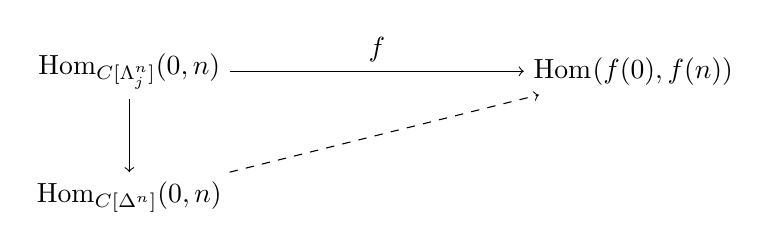
\begin{tikzpicture}
  \node (a) at (0,0)
    {$\mathrm{Hom}_{\mathfrak{C}[\Lambda^n_j]}(0, n)$};
  \node (b) at (6.4,0) {$\mathrm{Hom}_{\C}(f(0), f(n))$};
  \node (c) at (0,-1.6)
    {$\mathrm{Hom}_{\mathfrak{C}[\Delta^n]}(0, n)$};
  \draw[->] (a) -- node[above] {$f$} (b);
  \draw[->] (a) -- (c);
  \draw[->, dashed] (c) -- (b);
\end{tikzpicture}
\end{center}
由\cref{lem:c-lambda-n-j} 的描述与事实 1.1.48 可知，这个竖直映射是\trSimplicialSet{}之间的一个\trAnodyneMap{}。
（我们还将在引理 1.3.31 中给出一个独立的论证。）因此，虚线箭头存
在。现在只需证明这个构造事实上产生一个单纯\trFunctor{}%
$\mathfrak{C}[\Delta^n] \to \C$。为了看出这一点，我们利用
$\mathrm{Hom}_{\mathfrak{C}[\Delta^n]}(0, 0) = \Delta^0 = \mathrm{Hom}_{\mathfrak{C}[\Delta^n]}(n, n)$ 这一事实，
因此不需要验证任何新的\trFunctor{}性
关系：由于图表
\begin{center}
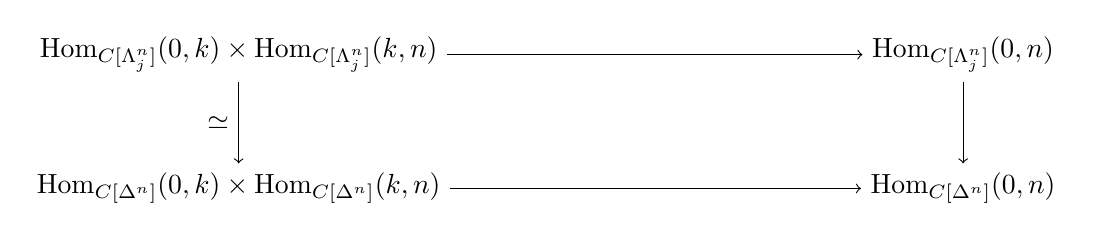
\begin{tikzpicture}
  \node (a) at (0,0) {$\mathrm{Hom}_{\mathfrak{C}[\Lambda^n_j]}(0, k) \times \mathrm{Hom}_{\mathfrak{C}[\Lambda^n_j]}(k, n)$};
  \node (b) at (9.2,0) {$\mathrm{Hom}_{\mathfrak{C}[\Lambda^n_j]}(0, n)$};
  \node (c) at (0,-1.7) {$\mathrm{Hom}_{\mathfrak{C}[\Delta^n]}(0, k) \times \mathrm{Hom}_{\mathfrak{C}[\Delta^n]}(k, n)$};
  \node (d) at (9.2,-1.7) {$\mathrm{Hom}_{\mathfrak{C}[\Delta^n]}(0, n)$};
  \draw[->] (a) -- (b);
  \draw[->] (a) -- node[left] {$\simeq$} (c);
  \draw[->] (b) -- (d);
  \draw[->] (c) -- (d);
\end{tikzpicture}
\end{center}
交换，那么任何穿过对象 $k$（$0 < k < n$）的合成都已经包含在子\trSimplicialCategory{}%
$\mathfrak{C}[\Lambda^n_j]$ 之中。
\end{proof}

\begin{observation}\label{obs:strict-2-category}
通过应用\trNerve{}，我们发现一个严格的 $2$-范畴产生一个\trSimplicialCategory{}，于
是其\trCoherentNerve{}是一个\trComposer{}。此外，一个严格的 $(2, 1)$-范畴产生一个所有
hom-单纯集都是\trGroupoid{}之\trNerve{}的\trSimplicialCategory{}，因而由%
\cref{lem:nerve-kan-iff-groupoid}，它们是\trKanComplex{}。特别地，一个严格的
$(2, 1)$-范畴在我们的意义下产生一个\trInfinityCategory{}。
\end{observation}

\begin{definition}\label{def:infinity-category-spaces}
考虑以 \trCWComplex{}为\trObject{}、hom-单纯集由\trMappingSpace{}的%
\trSingularSimplicialSet{}给出的那个\trSimplicialCategory{}。（注意，\trSingularSimplicialSet{}与积
交换。）这个范畴的单纯\trNerve{}给出一个\trInfinityCategory{}，我们称之为空间
∞-范畴，并记作 $\mathrm{Spc}$。
\end{definition}

\begin{observation}\label{obs:spc-objects}
$\mathrm{Spc}$ 的\trObject{}是 \trCWComplex{}，而其\trMorphism{}由空间
$\mathrm{map}(X, Y)$ 中的点给出，也就是说，由从 $X$ 到 $Y$ 的一个连续映射给出。
\trHomotopy{}范畴正如人们所期望的那样：\trMorphism{}是映射的\trHomotopy{}类。
\end{observation}

\begin{remark}\label{rem:purely-simplicial-model}
我们希望有空间∞-范畴的一个「纯单纯」模型（这话说来有点别扭——但它源于我们想把
Kan 复形/空间视为∞-\trGroupoid{}、并希望此后让空间与\trInfinityCategories{}处于平等
地位这一愿望），也就是说，一个我们直接构造以\trKanComplex{}为对象的%
\trSimplicialCategory{}的模型。为此，我们将需要证明：对一个\trSimplicialSet{} $K$
与一个\trKanComplex{} $X$，映射单纯集 $\underline{\mathrm{Hom}}(K, X)$ 仍是一个%
\trKanComplex{}。证明这一点所需的那些工具，在证明∞-\trGroupoid{}是\trKanComplex{}的
路途中也是必需的，而我们将在下一节开始建立这些工具。
\end{remark}

\begin{lemma}\label{lem:product-coproduct-infinity-categories}
\trInfinityCategories{}的积是一个\trInfinityCategory{}，而且\trInfinityCategories{}的
余积也是一个\trInfinityCategory{}。
\end{lemma}

\begin{proof}
对于积，可以在每个\trInfinityCategory{}中单独求解\trLiftingProblem{}，这便给出积的一个扩张。
对于余积，我们观察到 $\Lambda^n_j$ 与 $\Delta^n$ 都是连通的。因此，
\trInfinityCategories{}的余积的扩张问题实际上是单个\trInfinityCategory{}的扩张
问题。
\end{proof}

\begin{definition}\label{def:sub-infinity-category}
\trInfinityCategory{} $\C$ 的一个子∞-范畴 $\C'$ 是一个子单纯集，它由 $0$-\trSimplex{}的一个
子集 $X \subseteq \C_0$ 与由落在 $X$ 中的对象之间的 $1$-\trSimplex{}构成的一个子集
$S \subseteq \C_1$ 确定，使得 $S$ 包含恒等元并对合成与\trEquivalence{}封闭。于是，$\C$ 的一
个 $n$-\trSimplex{}属于 $\C'$，当且仅当它限制到\trSpine{} $I^n$ 上的那些边都包含在 $S$ 之
中。如果 $S$ 等于所有边界落在 $X$ 中的 $1$-\trSimplex{}之集，则称一个子范畴是\emph{满的}
（full）（在对象 $X \subseteq \C_0$ 上）。
\end{definition}

\begin{lemma}\label{lem:sub-infinity-category}
\trInfinityCategory{}的子∞-范畴本身是一个\trInfinityCategory{}。其\trHomotopy{}范畴
是 $h\C$ 中由位于 $S$ 中的\trMorphism{}的像所构成的子范畴。图表
\begin{center}
\begin{tikzpicture}
  \node (a) at (0,0) {$\C'$};
  \node (b) at (3,0) {$\C$};
  \node (c) at (0,-1.5) {$\mathrm{N}(h\C')$};
  \node (d) at (3,-1.5) {$\mathrm{N}(h\C)$};
  \draw[->] (a) -- (b);
  \draw[->] (a) -- (c);
  \draw[->] (b) -- (d);
  \draw[->] (c) -- (d);
\end{tikzpicture}
\end{center}
是一个\trPullback{}。此外，对\trHomotopy{}范畴的任何子范畴 $(h\C)' \subseteq h\C$，
这个\trPullback{}定义了 $\C$ 的一个子∞-范畴，其中 $X$ 与 $S$ 由沿典范映射
$\C \to \mathrm{N}(h\C)$ 的对象与\trMorphism{}的原像给出。
\end{lemma}

\begin{proof}
设 $\C$ 是一个\trInfinityCategory{}，并设 $\D \subseteq h\C$ 是其%
\trHomotopy{}范畴的一个子范畴。设 $\C'$ 是\trPullback{}%
$\mathrm{N}(\D) \times_{\mathrm{N}(h\C)} \C$。由于\trPullback{}保持\trMonomorphism{}，$\C'$ 是
$\C$ 的一个子单纯集。让我们详细说明 $\C$ 的一个 $n$-\trSimplex{}落在 $\C'$ 中意味着什么：
它恰好意味着 $\mathrm{N}(h\C)$ 中诱导的 $n$-\trSimplex{}落在 $\mathrm{N}(\D)$ 之中。
这当且仅当该\trSimplex{}的\trSpine{}（从而其每条边）落在 $\D$ 中时成立。现在注意，
一个包含 $X$ 中所有对象的恒等元、并对合成封闭的子集 $S \subseteq \C_1$ 事实上是
$h\C$ 的某个子范畴的\trNerve{}的 $1$-态射的原像。注意，在上面的定义中，我们有
$(\C')_1 = S$。
\end{proof}

\begin{corollary}\label{cor:subcat-correspondence}
在 $\C$ 的子∞-范畴与 $h\C$ 的子范畴之间存在一个由取\trHomotopy{}范畴诱导的
双射对应。$\C$ 的满子∞-范畴恰好对应于 $h\C$ 的满子范畴。
\end{corollary}

\begin{definition}\label{def:natural-transformation}
两个\trFunctor{} $f, g\colon \C \to \D$ 之间的一个\trNaturalTransformation{}是一个%
\trSimplicialMap{} $\C \times \Delta^1 \to \D$，其在两端的适当限制恰为给定的这两个\trFunctor{}。
\end{definition}

\begin{observation}\label{obs:hom-simplicial-infinity-category}
$X$ 与 $Y$ 之间的\trFunctor{}及其\trNaturalTransformation{}恰好是 hom-单纯集
$\underline{\mathrm{Hom}}(X, Y)$ 的 $0$-\trSimplex{}与 $1$-\trSimplex{}。如同在通常的%
\trCategoryTheory{}中一样，我们希望有一个由两个∞-范畴之间的\trFunctor{}构成的
∞-范畴。此外，人们会期望
$\mathrm{N}(\mathrm{Fun}(\C, \D)) = \mathrm{Fun}(\mathrm{N}\C, \mathrm{N}\D)$。由于\trNerve{}函子是%
\trFullyFaithful{}，我们还有
$\mathrm{N}(\mathrm{Fun}(\C, \D)) = \underline{\mathrm{Hom}}(\mathrm{N}\C, \mathrm{N}\D)$，
于是人们可以指望 hom-单纯集又是一个∞-范畴。这将被证明是真的，而且正如%
\trKanComplex{}的情形那样，这并非一件平凡事。接下来几节的目标之一就是证明这一事实。
\end{observation}
